\documentclass[10]{article}
%\documentclass[11pt]{book}
\usepackage{hyperref}
\usepackage{amsfonts,amssymb,amsmath,amsthm,cite}
%\usepackage{graphicx}
\usepackage[toc,page]{appendix}
\usepackage{nicefrac}
%% \usepackage[francais]{babel}
\usepackage[applemac]{inputenc}
\usepackage{amssymb, euscript}
\usepackage[matrix,arrow,curve]{xy}
\usepackage{graphicx}
\usepackage{tabularx}
\usepackage{float}
\usepackage{tikz}
\usepackage{slashed}
\usepackage{mathrsfs}
\usepackage{multirow}
\usepackage{rotating}

%\usepackage{mathtools}

\usetikzlibrary{matrix}
\usetikzlibrary{cd}

\usepackage{siunitx}

\usepackage{lmodern}
\usepackage[T1]{fontenc}
\usepackage[babel=true]{microtype}

\newcommand{\Wedgem}{\Wedge^{\mathrm{max}}}
\DeclareMathOperator{\inv}{inv}


\newcommand{\cs}{\mbox{\upshape C}\ensuremath{{}^*}} 
\newcommand{\csr}{{\mathrm C}^*_{\mathrm r}}
\newcommand{\csm}{\cs_{\mathrm{max}}}
\newcommand{\co}{\mathbb{C}}
\newcommand{\Grp}{\mathsf{G}}
\newcommand{\Sig}{{\sf\Sigma}}
\newcommand{\PI}{{\sf\Pi}}
\DeclareMathOperator{\Pair}{Pair}
\DeclareMathOperator{\Tw}{Tw}
\newcommand{\BS}{\text{B-S}}


\newcommand{\Alg}{\mathsf{A}}
\newcommand{\p}{\mathfrak{P}}


\DeclareMathOperator{\curv}{curv}

\def\bean#1\eean{\begin{equation}#1\end{equation}}
\newcommand{\s}{\mathsf{s}}
\renewcommand{\t}{\mathsf{t}}
\newcommand{\m}{\mathsf{m}}

 \newcommand{\fchoice}[2]{#2}
\DeclareMathSymbol{\onto}{\mathrel}{AMSa}{"10}
\renewcommand{\hbar}{{\mathchar'26\mkern-9muh}}
\newcommand{\Wedge}{\mathsf{\Lambda}}
\newcommand{\espace}{}

\DeclareMathOperator{\pr}{pr}


\usepackage{amsfonts,cite}
\usepackage{graphicx}

%% \usepackage[francais]{babel}
\usepackage[applemac]{inputenc}


\usepackage[sc]{mathpazo}
\usepackage{environ}

\linespread{1.05}         % Palatino needs more leading (space between lines)


%\usepackage[usenames]{color}



\DeclareFontFamily{T1}{pzc}{}
\DeclareFontShape{T1}{pzc}{m}{it}{1.8 <-> pzcmi8t}{}
\DeclareMathAlphabet{\mathpzc}{T1}{pzc}{m}{it}
\DeclareMathOperator{\cosupp}{\mathfrak{cosupp}}            %% 
% the command for it is \mathpzc

\textwidth=140mm


% % % % % % % % % % % % % % % % % % % %
\theoremstyle{plain}
\newtheorem{prop}{Proposition}[section]
\newtheorem{prdf}[prop]{Proposition and Definition}
\newtheorem{lem}[prop]{Lemma}%[section]
\newtheorem{cor}[prop]{Corollary}%[section]
\newtheorem{thm}[prop]{Theorem}%[section]
\newtheorem{theorem}[prop]{Theorem}
\newtheorem{lemma}[prop]{Lemma}
\newtheorem{proposition}[prop]{Proposition}
\newtheorem{corollary}[prop]{Corollary}
\newtheorem{statement}[prop]{Statement}

\theoremstyle{definition}
\newtheorem{defn}[prop]{Definition}%[section]
\newtheorem{cordefn}[prop]{Corollary and Definition}%[section]
\newtheorem{empt}[prop]{}%[section]
\newtheorem{exm}[prop]{Example}%[section]
\newtheorem{rem}[prop]{Remark}%[section]
\newtheorem{prob}[prop]{Problem}
\newtheorem{conj}{Conjecture}       %% Hypothesis 1
\newtheorem{cond}{Condition}        %% Condition 1
%\newtheorem{axiom}[thm]{Axiom}           %% Axiom 1 modified
\newtheorem{fact}[prop]{Fact}
\newtheorem{ques}{Question}         %% Question 1
\newtheorem{answ}{Answer}           %% Answer 1
\newtheorem{notn}{Notation}        %% Notations are not numbered

\theoremstyle{definition}
\newtheorem{notation}[prop]{Notation}
\newtheorem{definition}[prop]{Definition}
\newtheorem{example}[prop]{Example}
\newtheorem{exercise}[prop]{Exercise}
\newtheorem{conclusion}[prop]{Conclusion}
\newtheorem{conjecture}[prop]{Conjecture}
\newtheorem{criterion}[prop]{Criterion}
\newtheorem{summary}[prop]{Summary}
\newtheorem{axiom}[prop]{Axiom}
\newtheorem{problem}[prop]{Problem}
%\theoremstyle{remark}
\newtheorem{remark}[prop]{Remark}

\numberwithin{equation}{section}
\newtheorem*{claim}{Claim}
\DeclareMathOperator{\Dom}{Dom}              %% domain of an operator
\newcommand{\Dslash}{{D\mkern-11.5mu/\,}}    %% Dirac operator
\newcommand{\trG}{{\rm tr}_G\;}
\newcommand{\trF}{{\rm tr}_{\cal F}\;}
\newcommand{\TR}{{\rm TR}\;}
\newcommand{\res}{{\rm res}\;}


\newcommand\ci{${\mathcal C}^{\infty}$}
\newcommand\CI{{\mathcal C}^{\infty}}
\newcommand\CIc{{\mathcal C}^{\infty}_{\text{c}}}

%\newcommand\myeq{\stackrel{\mathclap{\normalfont\mbox{def}}}{=}}
\newcommand{\rar}[1]{\stackrel{#1}{\longrightarrow}}
\newcommand{\lar}[1]{\stackrel{#1}{\longleftarrow}}

\newcommand{\nor}[1]{\left\Vert #1\right\Vert}    %\nor{x}=||x||
\newcommand{\norm}[1]{\left\| #1\right\|}    %\nor{x}=||x||
\newcommand{\vertiii}[1]{{\left\vert\kern-0.25ex\left\vert\kern-0.25ex\left\vert #1
		\right\vert\kern-0.25ex\right\vert\kern-0.25ex\right\vert}}
\newcommand{\Ga}{\Gamma}  
\newcommand{\coker}{\mathrm{coker}}                   %% short for  \Gamma
\newcommand{\Coo}{C^\infty}                  %% smooth functions
\newcommand{\dom}{\mathrm{dom}}                  %% smooth functions
\newcommand{\Cont}{C} 
\newcommand{\cl}{\overline} 
\newcommand{\Contc}{C_c} 
\newcommand{\Contb}{C_b} 
\newcommand{\Repi}{\mathrm{Rep}_{int}} 
\newcommand{\Rep}{\mathrm{Rep}} 
\newcommand{\hor}[0]{\mathrm{hor}}
\newcommand{\comp}{\operatorname{comp}}
\newcommand{\adb}{\operatorname{adb}}
\newcommand{\dist}{\operatorname{dist}}


% % % % % % % % % % % % % % % % % % % %


\usepackage[sc]{mathpazo}
\linespread{1.05}         % Palatino needs more leading (space between lines)

\newbox\ncintdbox \newbox\ncinttbox %% noncommutative integral symbols
\setbox0=\hbox{$-$} \setbox2=\hbox{$\displaystyle\int$}
\setbox\ncintdbox=\hbox{\rlap{\hbox
		to \wd2{\hskip-.125em \box2\relax\hfil}}\box0\kern.1em}
\setbox0=\hbox{$\vcenter{\hrule width 4pt}$}
\setbox2=\hbox{$\textstyle\int$} \setbox\ncinttbox=\hbox{\rlap{\hbox
		to \wd2{\hskip-.175em \box2\relax\hfil}}\box0\kern.1em}

\newcommand{\ncint}{\mathop{\mathchoice{\copy\ncintdbox}%
		{\copy\ncinttbox}{\copy\ncinttbox}%
		{\copy\ncinttbox}}\nolimits}  %% NC integral

%%% Repeated relations:
\newcommand{\xyx}{\times\cdots\times}      %% repeated product
\newcommand{\opyop}{\oplus\cdots\oplus}    %% repeated direct sum
\newcommand{\oxyox}{\otimes\cdots\otimes}  %% repeated tensor product
\newcommand{\wyw}{\wedge\cdots\wedge}      %% repeated exterior product
\newcommand{\subysub}{\subset\hdots\subset}      %% repeated subset
\newcommand{\supysup}{\supset\hdots\supset}      %% repeated supset
\newcommand\CC{\mathbb C}
\newcommand\NN{\mathbb N}
\newcommand\RR{\mathbb R}
\newcommand\ZZ{\mathbb Z}
\newcommand{\LGR}{\matcal L}
\newcommand{\rep}{\mathfrak{rep}}
\newcommand{\lift}{\mathfrak{lift}}
\newcommand{\desc}{\mathfrak{desc}}
\newcommand{\Cstar}{C^*}
\newcommand{\Cst}{C^*}
\newcommand{\Star}{*}
\newcommand{\PS}[1]{\Psi^{#1}(\GR;E)}

%%% Roman letters:
\newcommand{\id}{\mathrm{id}}                %% identity map
\newcommand{\Id}{\mathrm{Id}}                %% identity map
\newcommand{\pt}{\mathrm{pt ???}}                %% a point
\newcommand{\const}{\mathrm{const}}          %% a constant
\newcommand{\codim}{\mathrm{codim}}          %% codimension
\newcommand{\cyc}{\mathrm{cyclic}}  %% cyclic sum
\renewcommand{\d}{\mathrm{d}}       %% commutative differential
\newcommand{\dR}{\mathrm{dR}}       %% de~Rham cohomology
\newcommand{\proj}{\mathrm{proj}}                %% a projection
\newcommand*{\braket}[2]{\langle#1 {,~} #2\rangle}% right inner products
\newcommand*{\lbraket}[2]{\langle\!\langle#1{\mid}#2\rangle\!\rangle}% left inner products

\newcommand*{\Mult}{\mathcal M}% multiplier algebra
\newcommand{\Lt}{\mathcal{L}}                 %%\newcommand{\unitsv}[1]{#1^{(0)}}

\newcommand{\A}{\mathcal{A}}                 %%\newcommand{\unitsv}[1]{#1^{(0)}}
\newcommand{\units}{G^{(0)}}
\newcommand{\haars}{\{\lambda^{u}\}_{u\in\units}}
\newcommand{\shaars}{\{\lambda_{u}\}_{u\in\units}}
\newcommand{\haarsv}[2]{\{\lambda^{#2}_{#1}\}_{#2\in\unitsv{#1}}}
\newcommand{\haarv}[2]{\lambda^{#2}_{#1}}

\renewcommand{\a}{\alpha}                    %% short for  \alphapha
\DeclareMathOperator{\ad}{ad}                %% infml adjoint repn
\newcommand{\as}{\quad\mbox{as}\enspace}     %% `as' with spacing
\newcommand{\Aun}{\widetilde{\mathcal{A}}}   %% unital algebra
\newcommand{\B}{\mathcal{B}}                 %% space of distributions
\newcommand{\E}{\mathcal{E}}                 %% space of distributions
\renewcommand{\b}{\beta}                     %% short for \beta
\newcommand{\braCket}[3]{\langle#1\mathbin|#2\mathbin|#3\rangle}
%\newcommand{\braket}[2]{\langle#1\mathbin|#2\rangle} %% <w|z>
\newcommand{\C}{\mathbb{C}}                  %% complex numbers
\newcommand{\cc}{\mathbf{c}}                 %% Hochschild cycle
\DeclareMathOperator{\Cl}{C\ell}             %% Clifford algebra
\newcommand{\F}{\mathcal{F}}                 %% space of test functions
\newcommand{\G}{\mathcal{G}}                 %% 
\newcommand{\GR}{\mathcal{G}}                 %% 
\newcommand{\D}{\mathcal{D}}                 %% Moyal L^2-filtration
\renewcommand{\H}{\mathcal{H}}               %% Hilbert space
\newcommand{\half}{\tfrac{1}{2}}             %% small fraction  1/2
\newcommand{\hh}{\mathcal{H}}                %% Hilbert space
\newcommand{\hookto}{\hookrightarrow}        %% abbreviation
\newcommand{\into}{\hookrightarrow}        %% abbreviation
\newcommand{\Ht}{{\widetilde{\mathcal{H}}}}  %% Hilbert space of forms
\newcommand{\I}{\mathcal{I}}                 %% tracelike functions
\DeclareMathOperator{\Junk}{Junk}            %% the junk DGA ideal
\newcommand{\K}{\mathcal{K}}                 %% compact operators
\newcommand{\ket}[1]{|#1\rangle}             %% ket vector
\newcommand{\ketbra}[2]{|#1\rangle\langle#2|} %% rank one operator
\renewcommand{\L}{\mathcal{L}}               %% operator algebra
\newcommand{\La}{\Lambda}                    %% short for \Lambda
\newcommand{\la}{\lambda}                    %% short for \lambda
\newcommand{\lf}{L_f^\theta}                 %% left  mult operator
\newcommand{\M}{\mathcal{M}}                 %% Moyal multplr algebra
\newcommand{\Lb}{\mathcal{L}}                 %% Moyal multplr algebra
\newcommand{\mm}{\mathcal{M}^\theta}
%\newcommand{{{\star_{\theta}}}{{\mathchoice{\mathbin{\;|\;ar_{_\theta}}}
			%            {\mathbin{\;|\;ar_{_\theta}}}           %% Moyal
			%            {{\;|\;ar_\theta}}{{\;|\;ar_\theta}}}}    %% product
	\newcommand{\N}{\mathbb{N}}                  %%  integers
	\newcommand{\nb}{\nabla}                     %% gradient
	\newcommand{\Oh}{\mathcal{O}}                %% comm multiplier alg
	\newcommand{\om}{\omega}                     %% short for \omega
	\newcommand{\opp}{{\mathrm{op}}}             %% opposite algebra
	\newcommand{\ox}{\otimes}                    %% tensor product
	\newcommand{\eps}{\varepsilon}                    %% tensor product
	\newcommand{\otimesyox}{\otimes\cdots\otimes}    %% repeated tensor product
	\newcommand{\pa}{\partial}                   %% short for \partial
	\newcommand{\pd}[2]{\frac{\partial#1}{\partial#2}}%% partial derivative
	\newcommand{\piso}[1]{\lfloor#1\rfloor}      %% integer part
	\newcommand{\PsiDO}{\Psi~\mathrm{DO}}         %% pseudodiffl operators
	\newcommand{\Q}{\mathbb{Q}}                  %% rational numbers
	\newcommand{\R}{\mathbb{R}}                  %% real numbers
	\newcommand{\rdl}{R_\Dslash(\lambda)}        %% resolvent
	\newcommand{\roundbraket}[2]{(#1\mathbin|#2)} %% (w|z)
	\newcommand{\row}[3]{{#1}_{#2},\dots,{#1}_{#3}} %% list: a_1,...,a_n
	\newcommand{\sepword}[1]{\quad\mbox{#1}\quad} %% well-spaced words
	\newcommand{\set}[1]{\{\,#1\,\}}             %% set notation
	\newcommand{\Sf}{\mathbb{S}}                 %% sphere
	\newcommand{\uhor}[1]{\Omega^1_{hor}#1}
	\newcommand{\sco}[1]{{\sp{(#1)}}}
	\newcommand{\sw}[1]{{\sb{(#1)}}}
	\DeclareMathOperator{\spec}{sp}              %% spectrum
	\renewcommand{\SS}{\mathcal{S}}              %% Schwartz space
	\newcommand{\sss}{\mathcal{S}}               %% Schwartz space
	\DeclareMathOperator{\supp}{\mathfrak{supp}}            %% support
	\newcommand{\T}{\mathbb{T}}                  %% circle as a group
	\renewcommand{\th}{\theta}                   %% short for \theta
	\newcommand{\thalf}{\tfrac{1}{2}}            %% small* fraction 1/2
	\newcommand{\tihalf}{\tfrac{i}{2}}           %% small* fraction i/2
	\newcommand{\tpi}{{\tilde\pi}}               %% extended representation
	\DeclareMathOperator{\Tr}{Tr}                %% trace of operator
	\DeclareMathOperator{\tr}{tr}                %% trace of matrix
	\newcommand{\del}{\partial}                  %% short for  \partial
	\DeclareMathOperator{\tsum}{{\textstyle\sum}} %% small sum in display
	\newcommand{\V}{\mathcal{V}}                 %% test function space
	\newcommand{\vac}{\ket{0}}                   %% vacuum ket vector
	\newcommand{\vf}{\varphi}                    %% scalar field
	\newcommand{\w}{\wedge}                      %% exterior product
	\DeclareMathOperator{\wres}{wres}            %% density of Wresidue
	\newcommand{\x}{\times}                      %% cross
	\newcommand{\Z}{\mathbb{Z}}                  %% integers
	\newcommand{\7}{\dagger}                     %% short for + symbol
	\newcommand{\8}{\bullet}                     %% anonymous degree
	\renewcommand{\.}{\cdot}                     %% anonymous variable
	\renewcommand{\:}{\colon}                    %% colon in  f: A -> B
	
	%\newcommand{\sA}{\mathscr{A}}       %%
	\newcommand{\sA}{\mathcal{A}} 
	\newcommand{\sB}{\mathcal{B}}       %%
	\newcommand{\sC}{\mathcal{C}}       %%
	\newcommand{\sD}{\mathcal{D}}       %%
	\newcommand{\sE}{\mathcal{E}}       %%
	\newcommand{\sF}{\mathcal{F}}       %%
	\newcommand{\sG}{\mathcal{G}}       %%
	\newcommand{\sH}{\mathcal{H}}       %%
	\newcommand{\sI}{\mathcal{I}}       %%
	\newcommand{\sJ}{\mathcal{J}}       %%
	\newcommand{\sK}{\mathcal{K}}       %%
	\newcommand{\sL}{\mathcal{L}}       %%
	\newcommand{\sM}{\mathcal{M}}       %%
	\newcommand{\sN}{\mathcal{N}}       %%
	\newcommand{\sO}{\mathcal{O}}       %%
	\newcommand{\sP}{\mathcal{P}}       %%
	\newcommand{\sQ}{\mathcal{Q}}       %%
	\newcommand{\sR}{\mathcal{R}}       %%
	\newcommand{\sS}{\mathcal{S}}       %%
	\newcommand{\sT}{\mathcal{T}}       %%
	\newcommand{\sU}{\mathcal{U}}       %%
	\newcommand{\sV}{\mathcal{V}}       %%
	\newcommand{\sX}{\mathcal{X}}       %%
	\newcommand{\sY}{\mathcal{Y}}       %%
	\newcommand{\sZ}{\mathcal{Z}}       %%
	
	\newcommand{\Om}{\Omega}       %%
	
	
	\DeclareMathOperator{\ptr}{ptr}     %% Poisson trace
	\DeclareMathOperator{\Trw}{Tr_\omega} %% Dixmier trace
	\DeclareMathOperator{\vol}{Vol}     %% total volume
	\DeclareMathOperator{\Vol}{Vol}     %% total volume
	\DeclareMathOperator{\Area}{Area}   %% area of a surface
	\DeclareMathOperator{\Wres}{Wres}   %% (Wodzicki) residue
	
	\newcommand{\dd}[1]{\frac{\partial}{\partial#1}}   %% partial derivation
	\newcommand{\ddt}[1]{\frac{d}{d#1}}                %% derivative
	\newcommand{\sfrac}[2]{{\scriptstyle\frac{#1}{#2}}} %% tiny fraction
	
	\newcommand\VD{{\mathcal D}}
	\newcommand{\bA}{\mathbb{A}}       %%
	\newcommand{\bB}{\mathbb{B}}       %%
	\newcommand{\bC}{\mathbb{C}}       %%
	\newcommand{\bCP}{\mathbb{C}P}     %%
	\newcommand{\bD}{\mathbb{D}}       %%
	\newcommand{\bE}{\mathbb{E}}       %%
	\newcommand{\bF}{\mathbb{F}}       %%
	\newcommand{\bG}{\mathbb{G}}       %%
	\newcommand{\bH}{\mathbb{H}}       %%
	\newcommand{\bHP}{\mathbb{H}P}     %%
	\newcommand{\bI}{\mathbb{I}}       %%
	\newcommand{\bJ}{\mathbb{J}}       %%
	\newcommand{\bK}{\mathbb{K}}       %%
	\newcommand{\bL}{\mathbb{L}}       %%
	\newcommand{\bM}{\mathbb{M}}       %%
	\newcommand{\bN}{\mathbb{N}}       %%
	\newcommand{\bO}{\mathbb{O}}       %%
	\newcommand{\bOP}{\mathbb{O}P}     %%
	\newcommand{\bP}{\mathbb{P}}       %%
	\newcommand{\bQ}{\mathbb{Q}}       %%
	\newcommand{\bR}{\mathbb{R}}       %%
	\newcommand{\bRP}{\mathbb{R}P}     %%
	\newcommand{\bS}{\mathbb{S}}       %%
	\newcommand{\bT}{\mathbb{T}}       %%
	\newcommand{\bU}{\mathbb{U}}       %%
	\newcommand{\bV}{\mathbb{V}}       %%
	\newcommand{\bX}{\mathbb{X}}       %%
	\newcommand{\bY}{\mathbb{Y}}       %%
	\newcommand{\bZ}{\mathbb{Z}}       %%
	
	\newcommand{\bydef}{\stackrel{\mathrm{def}}{=}}          %% 
	\newcommand{\defeq}{\stackrel{\mathrm{def}}{=}}   
	
	
	
	\newcommand{\al}{\alpha}          %% short for  \alpha
	\newcommand{\bt}{\beta}           %% short for  \beta
	\newcommand{\Dl}{\Delta}          %% short for  \Delta
	\newcommand{\dl}{\delta}          %% short for  \delta
	\newcommand{\ga}{\gamma}          %% short for  \gamma
	\newcommand{\ka}{\kappa}          %% short for  \kappa
	\newcommand{\sg}{\sigma}          %% short for  \sigma
	\newcommand{\Sg}{\Sigma}          %% short for  \Sigma
	\newcommand{\Th}{\Theta}          %% short for  \Theta
	\renewcommand{\th}{\theta}        %% short for  \theta
	\newcommand{\vth}{\vartheta}      %% short for  \vartheta
	\newcommand{\ze}{\zeta}           %% short for  \zeta
	
	\DeclareMathOperator{\ord}{ord}     %% order of a PsiDO
	\DeclareMathOperator{\rank}{rank}   %% rank of a vector bundle
	\DeclareMathOperator{\sign}{sign}   %%
	\DeclareMathOperator{\sgn}{sgn}   %%
	\DeclareMathOperator{\chr}{char}   %%
	\DeclareMathOperator{\ev}{ev}       %% evaluation
	
	\newcommand{\Op}{\mathbf{Op}}
	\newcommand{\As}{\mathbf{As}}
	\newcommand{\Com}{\mathbf{Com}}
	\newcommand{\LLie}{\mathbf{Lie}}
	\newcommand{\Leib}{\mathbf{Leib}}
	\newcommand{\Zinb}{\mathbf{Zinb}}
	\newcommand{\Poiss}{\mathbf{Poiss}}
	
	\newcommand{\gX}{\mathfrak{X}}      %% vector fields
	\newcommand{\sol}{\mathfrak{so}}    %% special orthogonal Lie algebra
	\newcommand{\gm}{\mathfrak{m}}      %% maximal ideal
	
	
	\DeclareMathOperator{\Res}{Res}
	\DeclareMathOperator{\NCRes}{NCRes}
	\DeclareMathOperator{\Ind}{Ind}
	%% co/homology theories
	\DeclareMathOperator{\rH}{H}        %% any co/homology
	\DeclareMathOperator{\rC}{C}        %%  any co/chains
	\DeclareMathOperator{\rZ}{Z}        %% cycles
	\DeclareMathOperator{\rB}{B}        %% boundaries
	\DeclareMathOperator{\rF}{F}        %% filtration
	\DeclareMathOperator{\Gr}{gr}        %% associated graded object
	\DeclareMathOperator{\rHc}{H_{\mathrm{c}}}   %% co/homology with compact support
	\DeclareMathOperator{\drH}{H_{\mathrm{dR}}}  %% de Rham co/homology
	\DeclareMathOperator{\cechH}{\check{H}}    %% Cech co/homology
	\DeclareMathOperator{\rK}{K}        %% K-groups
	\DeclareMathOperator{\rKO}{KO}        %% real K-groups
	\DeclareMathOperator{\rKU}{KU}        %% unitary K-groups
	\DeclareMathOperator{\rKSp}{KSp}        %% symplectic K-groups
	\DeclareMathOperator{\rR}{R}        %% representation ring
	\DeclareMathOperator{\rI}{I}        %% augmentation ideal
	\DeclareMathOperator{\HH}{HH}       %% Hochschild co/homology
	\DeclareMathOperator{\HC}{HC}       %% cyclic co/homology
	\DeclareMathOperator{\HP}{HP}       %% periodic cyclic co/homology
	\DeclareMathOperator{\HN}{HN}       %% negative cyclic co/homology
	\DeclareMathOperator{\HL}{HL}       %% Leibniz co/homology
	\DeclareMathOperator{\KK}{KK}       %% KK-theory
	\DeclareMathOperator{\KKK}{\mathbf{KK}}       %% KK-theory as a category
	\DeclareMathOperator{\Ell}{Ell}       %% Abstract elliptic operators
	\DeclareMathOperator{\cd}{cd}       %% cohomological dimension
	\DeclareMathOperator{\spn}{span}       %% span
	\DeclareMathOperator{\linspan}{span} %% linear span (can't use \span)
	\newcommand{\blank}{-}   
	
	
	
	\newcommand{\twobytwo}[4]{\begin{pmatrix} #1 & #2 \\ #3 & #4 \end{pmatrix}}
	\newcommand{\CGq}[6]{C_q\!\begin{pmatrix}#1&#2&#3\\#4&#5&#6\end{pmatrix}}
	%% q-Clebsch--Gordan coefficients
	\newcommand{\cz}{{\bullet}}         %% anonymous degree
	\newcommand{\nic}{{\vphantom{\dagger}}} %% invisible dagger
	\newcommand{\ep}{{\dagger}}         %% abbreviation for + symbol
	\newcommand{\downto}{\downarrow}    %% right hand limit
	\newcommand{\isom}{\cong}          %% isomorphism
	\newcommand{\lt}{\triangleright}    %% a left  action
	\newcommand{\otto}{\leftrightarrow} %% bijection
	\newcommand{\rt}{\triangleleft}     %% a right action
	\newcommand{\semi}{\rtimes}         %% crossed product
	\newcommand{\tensor}{\otimes}       %% tensor product
	\newcommand{\cotensor}{\square}       %% cotensor product
	\newcommand{\trans}{\pitchfork}     %% transverse
	\newcommand{\ul}{\underline}        %% for sheaves
	\newcommand{\upto}{\uparrow}        %% left  hand limit
	\renewcommand{\:}{\colon}           %% colon in  f: A -> B
	\newcommand{\blt}{\ast}
	\newcommand{\Co}{C_{\bullet}}
	\newcommand{\cCo}{C^{\bullet}}
	\newcommand{\nbs}{\nabla^S}         %% spin connection
	\newcommand{\up}{{\mathord{\uparrow}}} %% `up' spinors
	\newcommand{\dn}{{\mathord{\downarrow}}} %% `down' spinors
	\newcommand{\updn}{{\mathord{\updownarrow}}} %% up or down
	
	%%% Bilinear enclosures:
	
	\newcommand{\bbraket}[2]{\langle\!\langle#1\stroke#2\rangle\!\rangle}
	%% <<w|z>>
	\newcommand{\bracket}[2]{\langle#1,\, #2\rangle} %% <w,z>
	\newcommand{\scalar}[2]{\langle#1,\,#2\rangle} %% <w,z>
	\newcommand{\poiss}[2]{\{#1,\,#2\}} %% {w,z}
	\newcommand{\dst}[2]{\langle#1,#2\rangle} %% distributions <u,\phi>
	\newcommand{\pairing}[2]{(#1\stroke #2)} %% right-linear pairing
	\def\<#1|#2>{\langle#1\stroke#2\rangle} %% \braket (Dirac notation)
	\def\?#1|#2?{\{#1\stroke#2\}}        %% left-linear pairing
	
	%%% Accent-like macros:
	
	\renewcommand{\Bar}[1]{\overline{#1}} %% closure operator
	\renewcommand{\Hat}[1]{\widehat{#1}}  %% short for \widehat
	\renewcommand{\Tilde}[1]{\widetilde{#1}} %% short for \widetilde
	
	
	\DeclareMathOperator{\bCl}{\bC l}   %% complex Clifford algebra
	
	%%% Small fractions in displays:
	
	\newcommand{\ihalf}{\tfrac{i}{2}}   %% small fraction  i/2
	\newcommand{\quarter}{\tfrac{1}{4}} %% small fraction  1/4
	\newcommand{\shalf}{{\scriptstyle\frac{1}{2}}}  %% tiny fraction  1/2
	\newcommand{\third}{\tfrac{1}{3}}   %% small fraction  1/3
	\newcommand{\ssesq}{{\scriptstyle\frac{3}{2}}} %% tiny fraction  3/2
	\newcommand{\sesq}{{\mathchoice{\tsesq}{\tsesq}{\ssesq}{\ssesq}}} %% 3/2
	\newcommand{\tsesq}{\tfrac{3}{2}}   %% small fraction  3/2
	
	
	%\newcommand\eqdef{\over set{\mathclap{\normalfont\mbox{def}}}{=}}
	\newcommand\eqdef{\over set{\mathrm{def}}{=}}
	
	
	%+++++++++++++++++++++++++++++++++++
	
	\newcommand{\word}[1]{\quad\text{#1}\enspace} %% well-spaced words
	\newcommand{\words}[1]{\quad\text{#1}\quad} %% better-spaced words
	\newcommand{\su}[1]{{\sp{[#1]}}}
	
	\def\<#1,#2>{\langle#1,#2\rangle}            %% bilinear pairing
	\def\ee_#1{e_{{\scriptscriptstyle#1}}}       %% basis projector
	\def\wick:#1:{\mathopen:#1\mathclose:}       %% Wick-ordered operator
	
	\newcommand{\opname}[1]{\mathop{\mathrm{#1}}\nolimits}
	
	\newcommand{\hideqed}{\renewcommand{\qed}{}} %% to suppress `\qed'
	
	
	%%%%%%%%%%%%%%%%%%%%%%%%%%%%%
	%% 2. Some internal machinery
	%%%%%%%%%%%%%%%%%%%%%%%%%%%%%
	
	\newbox\ncintdbox \newbox\ncinttbox %% noncommutative integral symbols
	\setbox0=\hbox{$-$}
	\setbox2=\hbox{$\displaystyle\int$}
	\setbox\ncintdbox=\hbox{\rlap{\hbox
			to \wd2{\box2\relax\hfil}}\box0\kern.1em}
	\setbox0=\hbox{$\vcenter{\hrule width 4pt}$}
	\setbox2=\hbox{$\textstyle\int$}
	\setbox\ncinttbox=\hbox{\rlap{\hbox
			to \wd2{\hskip-.05em\box2\relax\hfil}}\box0\kern.1em}
	
	\newcommand{\disp}{\displaystyle} %% short for  \displaystyle
	
	%\newcommand{\hideqed}{\renewcommand{\qed}{}} %% no `\qed' at end-proof
	
	\newcommand{\stroke}{\mathbin|}   %% (for `\bbraket' and such)
	\newcommand{\tribar}{|\mkern-2mu|\mkern-2mu|} %% norm bars: |||
	
	%%% Enclose one argument with delimiters:
	
	\newcommand{\bra}[1]{\langle{#1}\rvert} %% bra vector <w|
	\newcommand{\kett}[1]{\lvert#1\rangle\!\rangle} %% ket 2-vector |y>>
	\newcommand{\snorm}[1]{\mathopen{\tribar}{#1}%
		\mathclose{\tribar}}                 %% norm |||x|||
	
	
	\newcommand{\End}{\mathrm{End}}       %%
	\newcommand{\Endo}{\mathrm{End}}       %%
	\newcommand{\Ext}{\mathrm{Ext}}       %%
	\newcommand{\Hom}{\mathrm{Hom}}       %%
	\newcommand{\Mrt}{\mathrm{Mrt}}       %%
	\newcommand{\grad}{\mathrm{grad}}       %%
	\newcommand{\Spin}{\mathrm{Spin}}       %%
	\newcommand{\Ad}{\mathrm{Ad}}       %%
	\newcommand{\Pic}{\mathrm{Pic}}       %%
	\newcommand{\Aut}{\mathrm{Aut}}       %%
	\newcommand{\Inn}{\mathrm{Inn}}       %%
	\newcommand{\Out}{\mathrm{Out}}       %%
	\newcommand{\Homeo}{\mathrm{Homeo}}       %%
	\newcommand{\Diff}{\mathrm{Diff}}       %%
	\newcommand{\im}{\mathrm{im}}       %%
	
	
	\newcommand{\SO}{\mathrm{SO}}       %%
	\newcommand{\SU}{SU}       %%
	\newcommand{\gso}{\mathfrak{so}}    %% special orthogonal Lie algebra
	\newcommand{\gero}{\mathfrak{o}}    %% orthogonal Lie algebra
	\newcommand{\gspin}{\mathfrak{spin}} %% spin Lie algebra
	\newcommand{\gu}{\mathfrak{u}}      %% unitary Lie algebra
	\newcommand{\gsu}{\mathfrak{su}}    %% special unitary Lie algebra
	\newcommand{\gsl}{\mathfrak{sl}}    %% special linear Lie algebra
	\newcommand{\gsp}{\mathfrak{sp}}    %% symplectic linear Lie algebra
	
	%\newcommand{\bes}{\begin{equation}\begin{split}}
			%\newcommand{\ees}{\end{split}\end{equation}}
	%\NewEnviron{split.enviro}{%
		%	\begin{equation}\begin{split}
				%	\BODY
				%	\end{split}\end{equation}
		%$}
	\newenvironment{splitequation}{\begin{equation}\begin{split}}{\end{split}\end{equation}}
	
	%Begin equation split: Begin equation split = bes
	\newcommand{\bs}{\begin{split}}
		\newcommand{\es}{\end{split}}
	\newcommand{\be}{\begin{equation}}
		\renewcommand{\ee}{\end{equation}}
	\newcommand{\bea}{\begin{eqnarray}}
		\newcommand{\eea}{\end{eqnarray}}
	\newcommand{\brray}{\begin{array}}
		\newcommand{\erray}{\end{array}}
	\newenvironment{equations}
	{\begin{equation}
			\begin{split}}
			{\end{split}
	\end{equation}}
	\newcommand{\Hsquare}{%
		\text{\fboxsep=-.2pt\fbox{\rule{0pt}{1ex}\rule{1ex}{0pt}}}%
	}
	\usetikzlibrary{calc,trees,positioning,arrows,chains,shapes.geometric,%
		decorations.pathreplacing,decorations.pathmorphing,shapes,%
		matrix,shapes.symbols}
	
	\usetikzlibrary{trees,positioning,shapes,shadows,arrows}
	
	
	\tikzset{
		basic/.style  = {draw, text width=2cm, drop shadow, font=\sffamily,     rectangle},
		root/.style   = {basic, rounded corners=2pt, thin, align=center,
			fill=green!30},
		level 2/.style = {basic, rounded corners=6pt, thin,align=center,     fill=green!60,
			text width=8em},
		level 3/.style = {basic, thin, align=left, fill=pink!60, text width=6.5em}
	}
	
	
	\title{Algebraic topology of $C^*$-algebras}
	
	\author
	{\textbf{Petr R. Ivankov*}\\
		e-mail: * monster.ivankov@gmail.com \\
	}
	
	
	\begin{document}
\maketitle  %\setlength{\parindent}{0pt}
\pagestyle{plain}

\begin{abstract}
	\noindent
\paragraph{}	Any $C^*$-algebra can be regarded as a generalization of locally compact Hausdorff topological space $\mathcal X$. Here we consider a generalization of fundamental group and (co)homology theory. In result one has invariants  of $C^*$-algebras such that: 
	\begin{itemize}
		\item for any commutative $C^*$-algebra $A = C_0\left(\sX \right)$ the invariants of $A$ coincide with the  $\sX$ ones,
		\item the theory is not trivial even for algebras having bad spectrum, e.g. containing  one point only.
	\end{itemize}
	Instead of $\sX$ we consider the space $\sY$ which should not be Hausdorff. However a noncommutative $C^*$-algebra $A$ defines $\sY$ and vice-versa.
	
\end{abstract}
\section{General Theory}
\subsection{The Gelfand space of $C^*$-algebra}




		\begin{definition}\label{upper_defn}\cite{johnstone:stone_spaces}
	Let $A$ be a partially ordered set, $S$ a subset of $A$. We say an element $a \in A$
is a \textit{ meet} (or \textit{ greatest lower bound}) for $S$, and write $a = \wedge S$, if 
\begin{enumerate}
	\item [(a)] $a$ is an lower bound for $S$, i.e. $a \le s$ for all $s \in S$ and, 
	\item [(b)] if $\forall s \in S\quad  b \le s$, then $b \le a$. 
\end{enumerate}
\paragraph{}
The antisymmetry axiom of the  partially ordered set $A$ ensures that the join of $S$, if it exists, is 
unique. If $S$ is a two-element set $\{s, t\}$, we write $s \wedge t$ for $\wedge \{s, t\}$ and if $S$	is the empty set $\emptyset$, we write $0$ for  $\wedge \emptyset$.
\end{definition}

\begin{definition}\label{lattice_defn}\cite{johnstone:stone_spaces}
	A \textit{meet-semilattice} is a partially ordered set which supports for any finite set the  greatest lower bound.
\end{definition}
\begin{definition}\label{filter_defn}\cite{johnstone:stone_spaces} 
	A subset $\mathfrak F$ of a meet-semilattice $A$ is said to be an {\it filter} if
	\begin{enumerate}
		\item [(a)] $\mathfrak F$ is a sub-meet-semilattice of $A$; i.e. $1\notin \mathfrak F$, and $a, b \in \mathfrak F$  imply  	$a \wedge b \in \mathfrak F$; and
		\item [(b)] $\mathfrak F$ is a lower set; i.e. $a \in \mathfrak F$ and $ a\le b$ imply $b \in \mathfrak F$.  
	\end{enumerate}
\end{definition}
\begin{empt}\label{filter_empt}
	Similarly to \cite{bourbaki_sp:gt} one has
	\begin{enumerate}
		\item [(c)] $0 \notin \mathfrak F$.
		
	\end{enumerate}	
	\begin{definition}
		A filter  $\mathfrak F$ is \textit{principal} if there is $b \in A$ such that 
		$$
		\mathfrak F = \left\{a \in A \left|~ b \le a\right.\right\}.
		$$
		
	\end{definition}
\end{empt}
\begin{remark}\label{fil_hom_rem}
	Any homomorphism $\phi : L' \to L''$ of {semi}-{lattices} yields a map
	of filers
\be\label{filtermap_eqn}
\left\{I_\la\right\}_{\la \in \La}	\mapsto \text{ minimal filter containing } \left\{\phi\left( I_\la\right) \right\}_{\la \in \La}
	\ee
\end{remark}

\begin{example}\label{space_semi_exm}
	If $\sX$ is a topological space then the $\sX$-\textit{semi}-\textit{lattice} is  a  meet-semilattice $\mathfrak{Lattice}\left( \sX\right)$ such that elements of $\mathfrak{Lattice}\left( \sX\right)$ are open subsets of $\sX$ and one has
	\be\label{x_lat_eqn}
\begin{split}
	\sU' \wedge \sU''\bydef \sU' \cap \sU'',\\
	\sU' \le \sU'' \quad \Leftrightarrow\quad \sU'' \subset \sU',\\
	0 \bydef \emptyset.
\end{split}
\ee
\end{example}


\begin{definition}\label{ultra_filter_defn}\cite{johnstone:stone_spaces} 
	A maximal filter is an \textit{ultrafilter}.
\end{definition}
\begin{remark}
			A set of neighborhoods of a point of Hausdorff space is an ultrafilter.
\end{remark}
\begin{thm}\label{zorn_thm}\cite{spanier:at} (Zorn's lemma). A partially ordered set in which every  simply ordered set has an upper bound contains maximal elements.
\end{thm}

\begin{remark}\label{ultra_filter_rem}
	From the Theorem \ref{zorn_thm} it follows that any filter is a subset of an	ultrafilter. (cf. \cite{johnstone:stone_spaces}).
\end{remark}

\begin{definition}\label{lattice_a_defn}
If $A$ be a $C^*$-algebra then $A$-\textit{semi}-\textit{lattice} is a meet-semilattice of closed left ideals such that 
\be\label{meet_eqn}
\begin{split}
L' \wedge L''\bydef L' \cap L'',\\
L' \le L'' \quad \Leftrightarrow\quad L' \subset L'',\\
0 \bydef \{0\}\subset A
\end{split}
\ee
We denote this semilattice by $\mathfrak{Lattice}\left( A\right)$ and denote by $\mathfrak{Filters}\left( A\right)$ a set of filers.
\end{definition}
\begin{thm}\label{gelfand-naimark_thm}\cite{arveson:c_alg_invt} (Commutative Gelfand-Na\u{\i}mark theorem). 
	Let $A$ be a commutative $C^*$-algebra and let $\mathcal{X}$ be the spectrum of A. There is the natural $*$-isomorphism $\gamma:A \xrightarrow{\cong} C_0(\mathcal{X})$.
\end{thm}
\begin{lemma}\label{top_lattices_iso_lem}
	For any locally compact space $\sX$ there is an isomorphism of  meet-semilattices
 
\be
\begin{split}
	\mathfrak{Lattice}_\sX : \mathfrak{Lattice}\left( C_0\left(  \sX\right)\right)\cong \mathfrak{Lattice}\left(\sX \right).
%	L \mapsto\sX \setminus \left\{x \in \sX | \forall a \in L \quad a(x) = 0\right\}.
\end{split}
\ee	
\end{lemma}
\begin{proof}
Any left ideal of  $C_0\left(  \sX\right)$ is a two-sided ideal. This lemma can be deduced from the proof of the Theorem \ref{gelfand-naimark_thm}.
\end{proof}
\begin{defn}\label{ultrafilters_space_defn}
 If $\mathfrak{Ultrafilters}\left(A \right)$ is a set of ultrafilters of the meet-semilattice $\mathfrak{Lattice}\left( A\right)$ then for any closed left ideal $L \subset A$ denote by
	\be\label{gelfand_eqn}
\mathfrak{Ultrafilters}\left(A \right)_L	\bydef \left\{\left. \xi \in \mathfrak{Ultrafilters}\left(A \right) \right| \exists L' \in \xi\quad L'\cap L = \{0\} \right\}
	\ee
	The \textit{space of} $A$-\textit{ultrafilters} is a set $\mathfrak{Ultrafilters}\left(A \right)$ with a  the smallest topology o such that any given by \eqref{gelfand_eqn} set is open.
	
\end{defn}
\begin{proposition}\label{top_ultra_thm}\cite{johnstone:stone_spaces}
	One has:
	\begin{enumerate}
		\item [(a)] 	A topological space $\sX$ is Hausdorff if and only if every ultrafilter on $\sX$ has at most one limit.
		\item[(b)]   	A topological space $\sX$ is compact if and only if every ultrafilter has at least one limit.
	\end{enumerate} 
\end{proposition}
\begin{remark}
From (b) of the Proposition \ref{top_ultra_thm} it follows that the notion of ultrafilter is not adequate analog of the point of Hausdorff, locally compact space. One needs the finer notion.
\end{remark} 
	\begin{thm}\label{pedersen_ideal_thm}  \cite{pedersen:ca_aut} 
	% THEOREM 5.6.1
	For each $C^*$-algebra $A$ there is a dense hereditary ideal $K(A)$,
	which is minimal among dense ideals.
	
\end{thm}
\begin{proof}
	Let $K(]0, \infty [)$ denote the set of continuous functions on $]0, \infty [$ with 
	compact support and define 
	\be\label{pedersen_k0_eqn}
	K\left( A \right)_0 \bydef \left\{f\left(x\right) \left|x \in A_+, \quad f \in K(]0, \infty [) \right.\right\}.
	\ee
	Let 
	\be\label{pedersen_k_plus_eqn}
	K\left( A \right)_+ \bydef \left\{x \in A_+ \left|x \le \sum_{j = 1}^nx_j, \quad x_j \in  	K\left( A \right)_0\right.\right\}, 	
	\ee
	so that $	K\left( A \right)_+$ is the smallest hereditary cone  containing $K\left( A \right)_0$. If $K(A)$ 
	is  the algebraic  $\C$-linear span of $K(A)_+$ then $K(A)$,
	which is minimal among dense ideals. The full  proof is  described in \cite{pedersen:ca_aut}.
\end{proof}

\begin{defn}\label{pedersen_ideal_defn}\cite{blackadar:ko}
	The ideal $K\left( A\right) $ from the theorem \ref{pedersen_ideal_thm} is said to be the {\it Pedersen's ideal of $A$}. %Henceforth Pedersen's ideal shall be denoted by $K(A)$.
\end{defn}
%\begin{remark}\label{pedersen_ideal_rem}
%	There is an explained in \cite{pedersen:mea_c} alternative definition  Pedersen's ideal. We think of the elements of $A$ as operators on its universal Hilbert space and denote by $A''$ the weak closure of $A$. A projection $p \in A''$ is called \textit{majorized} (relative to $A$) if there exists $b \in A_+$ such that $p \le b$. We let $\left[a\right]$ denote the range projection of any operator $a$ on a Hilbert space and define
%	\be\label{pedersen_ideal_eqn}
%	\begin{split}
%		K\left(A \right)_0  \bydef \left\{\left. a \in A_+ \right|  \left[a\right] \le b\right\},\\
%		K\left(A \right)_+  \bydef \left\{\left. a \in A_+ \right|\exists a_j \in K\left( A\right)_0 , ~ j = 1,...,n, ~ a \le \sum a_j \right\}.
%	\end{split}
%	\ee
%	$K\left(A \right)_0$ is a set of operators in $A_+$ with majorized supports, and $K\left(A \right)_+$ is the smallest ideal containing $K\left(A \right)_0$. The definition of $K\left(A \right)_0$ may be rephrased without reference to $A''$ as follows: $a \in K\left(A \right)_0$ if there exists $b\in A_+$ such that for all functions $\varphi$ continuous functions on the spectrum of $a$, $~0\le\varphi\le 1$ we have $\varphi\left( a\right) \le b$.	Pedersen's ideal $K\left(A\right)$ is the $\C$-linear span of $K\left(A \right)_0$.
%\end{remark}
\begin{remark}\cite{pedersen:ca_aut} 
	One has
	\bea\label{peder_k_eqn}
	K\left( \K\right) = \left\{\left. a \in \K\right| a  \text{ is a finite rank operator}\right\},\\
	\label{peder_c0_eqn}
	K\left(C_0\left(\sX \right)  \right) = C_c\left(\sX \right).
	\eea
	
\end{remark}	


\begin{definition}\label{gelfand_space_defn}
If $A$ is a $C^*$-algebra then	an ultrafilter  $\xi \in \mathfrak{Ultrafilters}\left(A \right)$ is a \textit{finite point} if there is a nontrivial element $a\in K\left( A\right)\setminus\{0\}$ such that 
	$$
  Aa \in \xi.
	$$
	The \textit{Gelfand space} $\mathfrak{Gelfand}\left(A \right)$ of $C^*$-algebra $A$ is a topological subspace  of the {space of} $A$-{ultrafilters} (cf. Definition \ref{ultrafilters_space_defn})
	$$
	\mathfrak{Gelfand}\left(A \right)\bydef \left\{\left. x \in \mathfrak{Ultrafilters}\left(A \right)\right| \exists L \in x \quad L \text{ is a finite point}\right\}.
	$$
\end{definition}


The following Lemma is a generalization of the Theorem \ref{gelfand-naimark_thm}.
\begin{lemma}\label{lem_g_lem} (Generalized commutative Gelfand theorem).
	If $\sX$ is a locally compact, Hausdorff space then  is a natural  homeomorphism $ \mathfrak{Gelfand}_\sX: \mathfrak{Gelfand}\left(C_0\left( \sX\right)  \right)\cong \sX$.
\end{lemma}
\begin{proof}
	From the Lemma \ref{top_lattices_iso_lem}  it turns out that for any locally compact space $\sX$ there is an isomorphism of  meet-semilattices
	
	\bean
	\begin{split}
		\mathfrak{Lattice}_\sX : \mathfrak{Lattice}\left( C_0\left(  \sX\right)\right)\cong \mathfrak{Lattice}\left(\sX \right).
		%	I \mapsto\sX \setminus \left\{x \in \sX | \forall a \in I \quad a(x) = 0\right\}.
	\end{split}
	\eean  
	It follows that there is a homeomorphism 
	$$
\mathfrak{Ultrafilters}_\sX : \mathfrak{Ultrafilters}\left( C_0\left(  \sX\right)\right)\cong \mathfrak{Ultrafilters}\left(\sX \right)
	$$ 	
	of spaces of ultrafilters. If $\xi \in \mathfrak{Ultrafilters}\left( C_0\left(  \sX\right)\right)$ then  denote by 
	$$
\sV_\xi\bydef 	\bigcap_{\sU \in \xi }\sU
	$$
	
	If $x \in \mathfrak{Gelfand}\left( C_0\left(  \sX\right)\right)$ then there if $a \in K\left( C_0\left( \sX\right) \right) \cong C_c\left( \sX\right)$ such that
	$$
aA \in \xi
	$$
or equivalently $\sV_\xi\subset  \supp a$.
	If 
	$$
\xi_a \bydef 	\left\{\left.\sU \cap \supp a \right| \sU \in\in \xi \right\}\in \mathfrak{Ultrafilters}\left( {\supp a}\right) 
	$$
	then  from the Proposition \ref{top_ultra_thm} it turns out that $\xi_a$ has the unique limit. This limit corresponds to $\mathfrak{Gelfand}_\sX\left( \xi\right)= \mathfrak{Gelfand}_{\supp a}\left( \xi_a\right)$.

\end{proof}
	\begin{lemma}\label{hered_ideal_lem}\cite{murphy}
	Let $A$ be a $C^*$-algebra.
	\begin{enumerate}
		\item[(i)] If $L$ is a closed left ideal in $A$ then $L\cap L^*$ is a hereditary $C^*$-subalgebra of $A$. The map $L \mapsto L\cap L^*$ is the bijection from the set of closed left deals of $A$ onto the the set of hereditary $C^*$-subalgebras of $A$.
		\item[(ii)] If $L_1, L_2$ are closed left ideals, then $L_1 \subseteq L_2$ is and only if $L_1\cap L_1^* \subset L_2\cap L_2^*$.
		\item[(iii)] If $B$ is a hereditary $C^*$-subalgebra of $A$, then the set 
		$$
		L\left(B \right) = \left\{\left.a \in A~\right| a^*a \in B \right\}
		$$
		is the unique closed left ideal of $A$ corresponding to $B$.
	\end{enumerate}
\end{lemma}


\begin{remark}\label{hered_ideal_rem}
	Using the Lemma \ref{hered_ideal_lem} one can replace the closed left ideals in the Definition \ref{gelfand_space_defn} with right ones or hereditary $C^*$-subalgebras. For any filter $\xi$7 we use a following notation
	\be\label{hered_ideal_eqn}
	L \in \xi \quad \Leftrightarrow \quad B \bydef L \cap L^* \in \xi\quad \Leftrightarrow \quad L^* \in \xi.
	\ee
\end{remark}

\begin{theorem}\label{left_ideal_thm}\cite{murphy}
	%3.1.2. Theorem.
	If $L$ is a closed left ideal in a $C^*$-algebra $A$, then there
	is an increasing net $\left\{u_\la\right\}_{\la\in\La}$ of positive elements in the closed unit ball of
	$L$ such that $a = \lim_{\la\in \La}au_\la $ for all $a\in L$.
\end{theorem}


\begin{definition}\label{bicommutant_defn}
Let $A$ be a $C^*$-algebra and let $L$ be a closed left ideal. The closed left ideal
$$
L^\perp \bydef \bigcup \left\{a \in A | L a^* = \{{0}\} \right\}
$$
is the \textit{commutant} of $L$ (write $L^\perp$),
For any element $\xi \in  \mathfrak{Filters} \left(A \right)$ the \textit{bicommutant} (written $\xi^{\perp\perp}$ or $\xi''$) is the closure of the union
$$
\bigcup_{L \in \xi} L^\perp.
$$
The set of bicommutants which are proper ideals (write $\mathfrak{Filters} \left(A \right)^{\perp\perp}$ $\mathfrak{Filters} \left(A \right)''$ is the \textit{bicommutant} of $\mathfrak{Filters} \left(A \right)$. The set of proper ideals which are bicommutants of the Gelfand space  (write $\mathfrak{Gelfand} \left(A \right)^{\perp\perp}$ $\mathfrak{Gelfand} \left(A \right)''$ is the \textit{bicommutant} of $\mathfrak{Gelfand} \left(A \right)$. There is the natural surjective  map 
\be\label{bicommutant_to_eqn}
 S \xrightarrow{\phi''}  \mathfrak{Gelfand} \left(A \right)''
\ee
from  the subset of $S \subset \mathfrak{Gelfand} \left(A \right)$ onto $\mathfrak{Gelfand} \left(A \right)''$. This map yields the initial topology (cf. Definition \ref{top_init_defn}), so the set $\mathfrak{Gelfand} \left(A \right)''$ is a topological space.
\end{definition}

\begin{example}
From the Lemma \ref{lem_g_lem} it follows that there is a homeomorphism $\mathfrak{Gelfand}_\sX: \mathfrak{Gelfand}\left(C_0\left( \sX\right)  \right)\cong \sX$. If $x = \mathfrak{Gelfand}_\sX\left( \xi\right)$ then for any $L \in \xi$ there is an open neighborhood of $x$ such that 
\bean
\forall a \in L \quad a\left(\sX \setminus \sU \right) = \{0\}
\eean  
so one has
\bean
\forall a \in L^\perp \quad a\left(\sU \right) = \{0\}
\eean

If $L_x \bydef \left\{a \in C_0\left(\sX \right) | a\left(x \right)= 0  \right\}$ 
the for any positive   $a'\in L_x$ one has
\be\label{pden_eqn}
\begin{split}
\left\|a' - f_{\eps/2}\left(a' \right)  \right\| < \eps,\\
\exists L \in \xi \quad a' \in L^\perp.\
\end{split}
\ee 
where $f_\eps$ is given by \eqref{f_eps_eqn}. From the equation \eqref{pden_eqn} it turns out that the subset of positive elements of the union $\cup  L^\perp$ is dense  in  the subset of positive elements of $L_x$.
If $A$ is a $C^*$-algebra then one has
\be\label{four_decompositon_eqn}
\forall a \in A\quad \exists a_1, a_2, a_3, a_4 \in A_+\quad a=a_1 - a_2 + ia_3 - ia_4 \quad  a_1, a_2, a_3, a_4 \ge 0.
\ee
From \eqref{four_decompositon_eqn} it follows that the the union $\cup  L^\perp$ is dense in $L_x$, so one has $L_x \subset \xi'' \bydef \phi''\left( \xi\right) $ (cf. Definition \ref{bicommutant_defn}). On the other hand if $a \notin L_x$ then $\left\|a\left(x \right)  \right\| > 0$ and
\bean
\forall L \in \xi \quad \exists a' \in L \quad a'\left(x \right)\neq 0 \quad  \Rightarrow \quad a'\left( x\right) a^*\left( x\right) \neq 0\quad  \Rightarrow \quad a'a^* \neq 0.
\eean 
So one has $\xi'' \subset L_x$, and  $\xi'' = L_x$. From this fact it turns out that the given by \eqref{bicommutant_to_eqn} map is a  homeomorphism from  $\mathfrak{Gelfand} \left(A \right)$ onto $ \mathfrak{Gelfand} \left(A \right)''$.
\end{example}

\begin{theorem}\label{irred_thm}\cite{pedersen:ca_aut}
	Let $\pi: A \to B\left(\H \right)$ be a nonzero representation of $C^*$-algebra $A$. The following conditions are equivalent:
	\begin{enumerate}
		\item [(i)] there are no non-trivial $A$-subspaces for $\pi$,
		\item[(ii)] the commutant of $\pi\left(A \right)$ is the scalar multipliers of 1,
		\item[(iii)] $\pi\left(A \right)$ is strongly dense in   $B\left(\H \right)$,
		\item[(iv)] for any two vectors $\xi, \eta \in \H$ with $\xi \neq 0$ there is $a \in A$ such that $\pi\left(a \right)\xi = \eta$,
		\item[(v)] each nonzero vector in $\H$ is cyclic for  $\pi\left(A \right)$,
		\item[(vi)]  $A \to B\left(\H \right)$ is spatially equivalent to a cyclic representation associated with a pure state of $A$.
	\end{enumerate} 
\end{theorem}
\begin{definition}\label{irred_defn}\cite{pedersen:ca_aut}
	Let $A \to B\left(\H \right)$ be a nonzero representation of $C^*$-algebra $A$. The representation is said to be \textit{irreducible} if it satisfies to the Theorem \ref{irred_thm}.
\end{definition}
\begin{definition}\label{spectrum_prime_primtive_defn}\cite{pedersen:ca_aut}
	An ideal $I$ in a $C^*$-algebra $A$ is \textit{prime}  if $xAy \subset I$  implies $x\in I$  or $y\in I$
	for all $x$, $y$ in $A$.  Equivalently, $I$ is prime if $I_1I_2\subset I$ implies  $I_1\subset I$ or 
	$I_2\subset I$ for any two (left, right, or two-sided) ideals $I_1$ and $I_2$ of $A$. 
	We say that $I$ is a \textit{primitive} ideal if $I= \ker\pi$ for some irreducible 
	representation $\pi: A \to B\left(\H \right)$. The set of prime ideals will be denoted by $\check{A}$ or $\mathrm{Prim}\left(A \right)$  and the set of primitive ideals will be denoted by $\hat A$. We say that $\check{A}$ is a \textit{prime spectrum} of $A$. The set  $\hat A$ is said to by a \textit{primitive  spectrum} or simply a \textit{spectrum} of $A$. For any $x \in \hat A$ denote  by $\rep_x: A \to B\left(\H_x\right)$ a corresponding irreducible representation. 
\end{definition}



\begin{definition}\label{belongs_defn}
	Let $A$ be a $C^*$ -algebra and let $\sY$ be the spectrum of $A$ (cf. Definition \ref{spectrum_prime_primtive_defn}). An element $\xi \in \mathfrak{Gelfand}\left(A \right)$  \textit{belongs to } $y \in \sY$ if one has
	\bean
	\forall L \in \xi \quad \rep_y\left(L^\perp \right) \neq \rep_y\left(A \right) 
	\eean
	where $\rep_y : A \to B\left(\H_y \right)$ is an irreducible representation (cf. Definition  \ref{irred_defn}).  Similarly the bicommutant $\xi''$ \textit{belongs to} $y$ if $\rep_y\left(\xi'' \right) \neq \rep_y\left(A \right)$.
	
\end{definition}
\begin{remark}
	Under the hypothesis of the Definition \ref{belongs_defn}  if $y', y'' \in \sY$ with $y' \neq y''$ and $\xi\in \mathfrak{Gelfand}\left(A \right)$ belongs to both $y'$, and $y''$ then the generated by the set $\left\{ L \cap \ker_{y'}\right\}$ filter exceeds $\xi$. It is impossible since $\xi$ is an ultrafilter.
	So there are natural maps:
	\be\label{to_spec_eqn}
	\begin{split}
		S \to \sY,\\
		S'' \to \sY,
	\end{split}
	\ee
	where $S\subset \mathfrak{Gelfand}\left(A \right)$ and $S''\subset \mathfrak{Gelfand}\left(A \right)''$ are subsets.
\end{remark}

\subsection{Morphisms}

\begin{definition}\label{lrc_defn}\cite{matro:hcm}
	If $A$ is a $C^*$-algebra then a linear map $\la: A\to A$ is said to be a \textit{left centralizer} if one has
	\be
	\la\left(ab\right)= 	\la\left(a\right) b \quad \forall a, b \in A.
	\ee
	Similarly one defines a \textit{right centralizer}. Denote the spaces of left and right centralizers by $\mathbf{LC}(A)$ and  $\mathbf{RC}(A)$.
\end{definition}
\begin{empt}
If both $A$ and $\widetilde{A}$ are $C^*$-algebra then any injective  homomorphism 	
\be\label{phi_r_eqn}
\varphi_R: A \hookto \mathbf{RC}\left(\widetilde A\right)	
\ee
of $\C$-algebras such that
\be\label{closed_p_eqn}
\widetilde{ A }\quad \text{is the closure of} \quad \widetilde A \varphi_R\left( A\right).
\ee
yields an injective homomorphism  
\be\label{lat_mor_eqn}
\begin{split}
	\mathfrak{Lattice}\left(  A\right) \xrightarrow{\mathfrak{Lattice}\left(\varphi_R \right)}\mathfrak{Lattice} \left( \widetilde A\right),\\
	L \mapsto \text{ the closure of } \widetilde A \varphi_R\left(L \right).
	\end{split}
	\ee
	On the other hand the homomorphism $\mathfrak{Lattice}\left(\varphi_R \right)$ yields a mapping of filters
\be\label{fil_mor_eqn}
\begin{split}
	\mathfrak{Filters}\left(  A\right) \xrightarrow{\mathfrak{Filters}\left(\varphi_R \right)}\mathfrak{Filters} \left( \widetilde A\right),\\
	\left\{L_\la\right\}_{\la \in \La} \mapsto \text{ a filter generated by } \bigcup_{\la \in \La} \left\{\mathfrak{Lattice}\left(\varphi_R \right)\left( L_\la\right) \right\}_{\la \in \La}
\end{split}
\ee
If $\xi \in \mathfrak{Ultrafilters}\left(  A\right) $ is an ultrafilter then we define a set
\bean
\mathfrak{Ultrafilters}\left(\varphi_R \right)^{-1}\left(\xi \right) \bydef\left\{\left.\widetilde \xi \in \mathfrak{Ultrafilters}\left(\widetilde  A\right)\right|\forall \widetilde{L}'\in \mathfrak{Filters}\left(\varphi_R \right)\left( \xi\right)\subset \widetilde \xi \right\}
\eean
For all $\xi', \xi''\in \mathfrak{Ultrafilters}\left(A \right)$ with $\xi' \neq \xi''$ there are $L' \in \xi'$ and $L'' \in \xi''$ such that $L'\cap L'' = \{0\}$. It turns out that
\bean
\xi', \xi''\in \mathfrak{Ultrafilters}\left(A \right)\quad \xi' \neq \xi'' \quad \Rightarrow\\
\Rightarrow \quad \mathfrak{Ultrafilters}\left(\varphi_R \right)^{-1}\left(\xi' \right)\cap \mathfrak{Ultrafilters}\left(\varphi_R \right)^{-1}\left(\xi ''\right)= \emptyset
\eean 
Using the above map one can construct the natural map
\be\label{ultra_mor_eqn}
\begin{split}
	\mathfrak{Ultrafilters}\left(\widetilde  A\right) \xrightarrow{\mathfrak{Ultrafilters}\left(\varphi_R \right)}\mathfrak{Ultrafilters} \left( A\right),\\
	\mathfrak{Ultrafilters}\left(\varphi_R \right)\left( \widetilde \xi\right) = \xi \quad \Leftrightarrow \quad \widetilde \xi \in \mathfrak{Ultrafilters}\left(\varphi_R \right)^{-1}\left(\xi \right).
\end{split}
\ee
\end{empt}
\begin{lemma}\label{good_lem}
The equation \eqref{fil_mor_eqn}  induces a continuous map.

\end{lemma}
\begin{proof}
 From the equation \eqref{gelfand_eqn} one can deduce any closed set on  that $\mathfrak{Ultrafilters}\left(A\right)$ corresponds to a closed set on $\mathfrak{Ultrafilters}\left(\widetilde A\right)$ 
\end{proof}.
\begin{defn}\label{good_defn}
The injective homomorphism \eqref{lat_mor_eqn} is \textit{good} if the given by \eqref{ultra_mor_eqn} map $\mathfrak{Ultrafilters}\left(\varphi_R \right)$ yields the natural continuous  map
	\be\label{gelfand_map_eqn}
\mathfrak{Gelfand}\left(\widetilde A \right)\xrightarrow{\mathfrak{Gelfand}\left(\varphi_R \right)}\mathfrak{Gelfand}\left(A \right).
\ee
\end{defn}
\begin{empt}\label{bicommutant_empt}
	Let $\varphi_R: A \hookto \mathbf{RC}\left(\widetilde A\right)$ be a good morphism. If $\widetilde \xi \in \mathfrak{Gelfand}\left(\widetilde A \right)$ and 
  $\widetilde \xi'' \in \mathfrak{Gelfand}\left(\widetilde A \right)''$ is the corresponding element  of bicommutant (cf. Definition \ref{bicommutant_defn} then there is $\widetilde{a}\in \widetilde{\xi}''$ end $\eps > 0$ such that
  \be\label{b_neq_eqn}
  \forall a_1, ..., a_n \in \xi'' \quad \forall \widetilde a_1, ..., \widetilde a_n \in A\quad \left\| \sum_{j =1}^n \widetilde a_j a_j - \widetilde a,\right\| > \eps.
  \ee
 where $\xi''$ is the bicommutant of  $\xi = \mathfrak{Gelfand}\left(\varphi_R \right) \left(\widetilde \xi \right)$. From
 \bean
 \forall L \in \xi \quad \text{the closure of } \widetilde A \varphi_R\left( L\right) \in \widetilde \xi.
 \eean 
it follows that 
 \bean
 \forall L \in \xi \quad \exists \widetilde L \in \widetilde \xi \quad \widetilde A   \varphi\left(L^\perp \right) \subset \widetilde L^\perp.
 \eean 
 If the closure $L'$ of the union 
 $$
 \bigcap_{L \in \xi} L^\perp 
 $$
 is not proper ideal the for any $a \in A$ and $\dl > 0$ there is $a' \in L'$  such that $\left\| a - a' \right\|< \dl$. If  $a'_1, ..., a'_n \in L'$ such that
 \bean
 \left\| a_j - a'_j \right\| < \frac{\eps}{n \left\|\widetilde  a_j  \right\|}
 \eean 
 then
 $$
 \left\| \sum_{j =1}^n \widetilde a_j a_j - \widetilde a,\right\| < \eps
 $$
 Above equation contradicts with \eqref{b_neq_eqn} one.
\end{empt}
\begin{lemma}\label{bicommutant_lem}
Any good morphism $\varphi_R: A \hookto \mathbf{RC}\left(\widetilde A\right)$ yields a continuous map
\be\label{bicommutant_eqn} 
\mathfrak{Gelfand}\left(\widetilde A \right)''\xrightarrow{\mathfrak{Gelfand}\left(\varphi_R \right)''}\mathfrak{Gelfand}\left(A \right)''.
\ee
\end{lemma}
\begin{proof}
The existence of the map follows from \ref{bicommutant_empt}. The continuity can be deduced from the continuity of $\mathfrak{Gelfand}\left(\varphi_R \right)$.
\end{proof}
\subsection{Coverings and fundamental group}
\subsubsection{Topologies of *-automorphisms groups}

If $A$ is a $C^*$-algebra then the group  $\mathrm{Aut}(A)$ of $*$-automorphisms carries several topologies making it into a topological group \cite{thomsem:ho_type_uhf}. The most important is {\it the topology of pointwise norm-convergence} based on the open sets
\begin{equation*}
	\left\{\left.\alpha \in \mathrm{Aut}(A) \ \right| \ \|\alpha(a)-a\| < 1 \right\}, \quad a \in A.
\end{equation*}
The other topology is the {\it uniform norm-topology} based on the open sets
\begin{equation}\label{aut_norm_eqn}
	\left\{\alpha \in \mathrm{Aut}(A) \ \left| \ \sup_{a \neq 0}\ \|a\|^{-1} \|\alpha(a)-a\| < \varepsilon \right. \right\}, \quad \varepsilon > 0
\end{equation}
which corresponds to following "norm"
\begin{equation}\label{uniform_norm_topology_formula_eqn}
	\|\alpha\|_{\text{Aut}} = \sup_{a \neq 0}\ \|a\|^{-1} \|\alpha(a)-a\| = \sup_{\|a\| =1}\  \|\alpha(a)-a\|.
\end{equation}
Above formula does not really means a norm because $\mathrm{Aut}\left(A\right)$ is not a vector space. Both of them can be used for our purposes.
\subsubsection{Basic construction}
\begin{definition}\label{connected_c_a_defn}
	We say that a $C^*$-algebra $A$ is \textit{connected} if it cannot be represented as a direct sum  $A \cong A' \oplus A''$ of nontrivial $C^*$-algebras $A'$ and $A''$.
	
	% (the Gelfand spectrum of the center of $M\left( A\right) $ is connected). Let $A \subset B$ be a connected subalgebra. We say that $A$ is a \textit{connected component} of $B$ if  $1_{M\left( A\right) }$ lies in the center of $1_{M\left( B\right) }$.
\end{definition}
\begin{definition}\label{fin_pre_defn}
	Let   $A$ be an unital connected $C^*$-algebra  and let  $\widetilde{A}$ be  connected $C^*$-algebra (cf. Definition \ref{connected_c_a_defn}), and let $\lift: A \hookto M\left( \widetilde{A}\right) $ be an injective  $*$-homomorphism of % connected
	$C^*$-algebras such that following conditions hold:
	\begin{enumerate}
		\item[(a)] $\lift\left( 1_A\right) = 1_{ M\left( \widetilde{A}\right)}$,
		\item[(b)] if $\Aut\left(\widetilde{A} \right)$ is a group of $*$-automorphisms of $\widetilde{A}$ then the group  
		\be\nonumber
		G \bydef \left\{ \left.g \in \Aut\left(\widetilde{A} \right)~\right|\forall a \in \lift \left(M\left(  A\right) \right) \quad ga = a\right\}
		\ee
		is discrete,
		\item[(c)] 	$A = M\left( \widetilde{A}\right) ^G\stackrel{\text{def}}{=}\left\{\left.a\in \widetilde{A}~~\right|\forall g \in G\quad  a = g a\right\}$.
	\end{enumerate}
	We say that the triple $\left(A, \widetilde{A}, G \right)$ and/or the quadruple $\left(A, \widetilde{A}, G, \lift \right)$ and/or $*$-homomorphism $\lift: A \hookto M\left( \widetilde{A}\right) $   is a \textit{noncommutative  pre-covering}. We write $G\left(\left.\widetilde A~\right|A \right)\bydef G$.
\end{definition}
	\begin{defn}\label{strict_topology_defn}\cite{pedersen:ca_aut}
	Let $A$ be a $C^*$-algebra.  The {\it strict topology} on the multiplier algebra $M(A)$ is the topology generated by seminorms 
	\be\label{strict_topology_norm_eqn}
	\vertiii{x}_a\bydef \|ax\| + \|xa\|,\quad a\in A.
	\ee
	If $\La$ is a directed set and $\left\{a_\la\in M\left( A\right) \right\}_{\la\in \La}$ is a net the we denote by $\bt\text{-}\lim_{\la\in\La }a_\la$ the limit of $\left\{a_\la \right\}$ with respect to the strict topology.
	If $x \in M(A)$  and a sequence of partial sums $\sum_{i=1}^{n}a_i$ ($n = 1,2, ...$), ($a_i \in A$) tends to $x$ in the strict topology then we shall write
	\begin{equation}\label{strict_topology_eqn}
		x = \bt\text{-}\sum_{i=1}^{\infty}a_i.
	\end{equation}
\end{defn}

\begin{definition}\label{evenly_defn}
	
	Let $\left(A, \widetilde{A}, G, \lift \right)$ be a noncommutative  pre-covering (cf. Definition \ref{fin_pre_defn})
	A connected hereditary $C^*$-subalgebra $B \subsetneqq A$ 
	is $\left(A, \widetilde{A}, G, \lift \right)$- \textit{evenly covered by} $\left(A, \widetilde{A}, G, \lift \right)$ if there is a hereditary $C^*$-subalgebra $\widetilde B \subset \widetilde A$ with a $*$-isomorphism $\lift^{\widetilde B}: B \cong \widetilde B$ such that
	\be\label{evenly_eqn}
	\forall b \in B \quad \lift\left( b\right) = \bt \text{-}\sum_{g\in G} g \lift^{\widetilde B}\left( b\right) 
	\ee
	where $\bt \text{-}\sum$ means the convergence with respect to the strict topology of $M\left( \widetilde A\right)$ (cf. the Definition \ref{strict_topology_defn} and the equation \eqref{strict_topology_eqn}).	
\end{definition}

\begin{definition}\label{cov_unital_defn}
	
	A  noncommutative  pre-covering $\left(A, \widetilde{A}, G, \lift \right)$ (cf. Definition \ref{fin_pre_defn}) with unital $A$ is a {\it unital noncommutative covering} if for any $x \in \mathfrak{Gelfand}\left(A \right)$ there is a hereditary connected $C^*$-subalgebra of $B$ {evenly covered by} $\left(A, \widetilde{A}, G, \lift \right)$ with $B \in x$
\end{definition}

\begin{definition}\label{cov_defn}
	Let $\left(A, \widetilde{A}, G, \lift \right)$ be a quadruple such that both $A$ and $\widetilde{A}$ are $C^*$-algebras $G \subset \Aut\left( \widetilde{A}\right)$ is a discrete subgroup and $\lift: A \hookto M\left( \widetilde{A}\right)$ is an injective $*$-homomorphism. If there is an unital noncommutative covering $\left(B, \widetilde{B}, G, \widetilde\lift \right)$  with inclusions $A \subset B$ and $\widetilde A \subset \widetilde B$ such that:
	\begin{enumerate}
		\item [(a)] both $A$ and $\widetilde A$ are essential ideals of $B$ and $\widetilde B$,
		\item[(b)] $\lift \bydef \left.\widetilde\lift\right|_A$,
		\item[(c)] the action $G \times \widetilde B \to \widetilde B$ naturally comes from the $G \times \widetilde A \to \widetilde A$.
	\end{enumerate}	
	then $\left(A, \widetilde{A}, G, \lift \right)$ is a \textit{noncommutative covering}.
\end{definition}

	


\begin{definition}\label{fund_den}
	If $A$ is a $C^*$ -algebra then a noncommutative covering $\left(A, \widetilde{A}, G, \lift \right)$ is \textit{universal}, if for any noncommutative covering $\left(A, \widetilde{A}', G', \lift' \right)$ there is natural noncommutative covering $\left(\widetilde{A}', \widetilde{A}, G'', \lift'' \right)$ with $\lift = \lift''\circ \lift'$. If the universal covering exists then $G$ is said to be the \textit{fundamental group} of $A$.
\end{definition}
	

\section{Applications}
\subsection{Fundamental group of commutative $C^*$-algebras}
\paragraph{} If $\sX$ is a connected, locally compact, Hausdorff space then there is a homeomorphism $\mathfrak{Gelfand}\left(C_0\left(\sX \right)  \right)\cong \sX$. If  $\left(C_0\left(\sX \right), \widetilde{A}, G, \lift \right)$ is a noncommutative covering then there is the given by  \ref{gelfand_map_eqn} continuous map
$$
\mathfrak{Gelfand}\left(\lift \right): \mathfrak{Gelfand}\left(\widetilde A \right)\to \sX.
$$
	
\begin{proposition}\label{hered_spectrum_prop}\cite{pedersen:ca_aut}
	If $B$ is a hereditary $C^*$-subalgebra of $A$ then the map $t \mapsto t\cap B$ is a homeomorphism between $\check A\setminus \mathrm{hull}\left( B\right)$ and $\check B$, where 
	$$
	\mathrm{hull}\left( B\right) = \left\{\left. x \in \hat A~\right|~ \rep_x\left(B \right)= \{0\} \right\} .
	$$ 
	Moreover  we have a commutative diagram:
	\\
	\begin{tikzcd}
		\hat A \setminus \mathrm{hull}\left(B \right)\arrow[d]\arrow[r, "\approx"] & \hat B\arrow[d]\\
		\check A \setminus \mathrm{hull}\left(B \right)\arrow[r, "\approx"] & \check B
	\end{tikzcd}
	\\ 	
\end{proposition}


%\begin{theorem}\label{ideal_spectrum_thm}\cite{pedersen:ca_aut}
	%4.1.11. THEOREM. 
%	Let $I$ be a closed ideal of $A$.
%	\begin{enumerate}
%		\item [(i)] The maps $\left(\pi: A \to B\left(\H \right)\right)   \mapsto \left(\pi|_L: L \to B\left(\H \right)\right)$ and \\$\left(\pi: A \to B\left(\H \right)\right)   \mapsto \left(\pi: A/L \to B\left(\H \right)\right)$ from 		$\mathrm{Lrr} A \setminus \mathrm{hull}\left( L\right)$  to $\mathrm{Lrr} L$ and from $\mathrm{hull}\left( L\right)$ to $\mathrm{Lrr} A/L$, respectively, induce 		isomorphisms 	$\hat A \setminus \mathrm{hull}\left( L\right)$  onto $\hat L$ and from $\mathrm{hull}\left( L\right)$ onto $\left( A/L\right)\hat~ $ 
%		\item[(ii)] The maps $t \mapsto t\cap L$ and $t \mapsto t/L$ are homeomorphisms from $\check{A}\setminus \mathrm{hull}\left(L \right)$  onto $\check{L}$ and from $\mathrm{hull}\left( L\right)$ onto $\left( A/L\right)\check~$.
	%	\item[(iii)] The resulting diagrams, below, are commutative:
%		\newline
%		\begin{tikzpicture}
%			\matrix (m) [matrix of math nodes,row sep=3em,column sep=4em,minimum width=2em]
%			{
%				\hat I   & \hat A\setminus \mathrm{hull}\left( I\right),  &\mathrm{hull}\left( I\right) &	\left( A/I\right)\hat~ \\ 
%				\check I  &  \check A\setminus \mathrm{hull}\left( I\right), & \mathrm{hull}\left( I\right) & 	\left( A/I\right)\check~\\};
%			\path[-stealth]
%			(m-1-2) edge node [above] {$\approx $} (m-1-1)
%			(m-1-3) edge node [above] {$\approx$} (m-1-4)
%			(m-2-2) edge node [above] {$\approx$} (m-2-1)
%			(m-2-3) edge node [above] {$\approx$} (m-2-4)
%			(m-1-1) edge node [right]  {} (m-2-1)
%			(m-1-2) edge node [right]  {} (m-2-2)
%			(m-1-3) edge node [right] {} (m-2-3)
%			(m-1-4) edge node [right] {} (m-2-4);
%		\end{tikzpicture}
%		\\ 	
		
%	\end{enumerate}
	
%\end{theorem}

	If $B\subset A$  is a hereditary $C^*$-subalgebra evenly covered by $\left(C_0\left(\sX \right), \widetilde{A}, G, \lift \right)$ (cf. Definition \ref{evenly_defn}) then there is a connected open subset $\sU \subset \sX$ with $B \cong \sU$. From the Definition \ref{evenly_defn} it follows that $\mathfrak{Gelfand}\left(\lift \right)^{-1}\left(\sU\right)$ is the disjoint union of homeomorphic to $\sU$ connected open subsets of  $\mathfrak{Gelfand}\left(\widetilde A \right)$, i.e. the map $\mathfrak{Gelfand}\left(\lift \right)$ is a covering. If $\widetilde A$ is not commutative then there is $\widetilde x \in \mathfrak{Gelfand}\left(\lift \right)$ with
	$$
\dim \widetilde A / \widetilde x > 1.	
	$$. From the condition (b) of the Definition \ref{fin_pre_defn} it follows that 
	$$
\dim C_0\left( \sX\right) / \mathfrak{Gelfand}\left(\lift \right)\left( \widetilde x\right) > 1.	
	$$
	It is impossible so $\widetilde A\cong C_0\left(\mathfrak{Gelfand}\left(\widetilde A\right) \right)$ is a commutative $C^*$-algebra. Thus there is an 1-1 correspondence between topological and noncommutative coverings of $C_0\left(\sX \right)$. From the Definition \ref{fund_den} that the fundamental group of $C_0\left(\sX \right)$ if it exists is isomorphic to $\pi_1\left( \sX\right)$. 
	\subsection{$C^*$-algebras of compact operators}

	
\paragraph{} If $\H$ is a Hilbert space and $A = \K\left(\H \right)$ then for any  left ideal $L\subset A$ there is a closed $\C$-linear subspace $V_L \subset \H$ such that
\bean
L = \left\{\left.a \in \K\left(\H \right)\right| a \H  \subset V_L\right\}.
\eean
If $L$ is minimal then $V_L$ is a one dimensional space. Any ultrafilter of the $\mathfrak{Lattice}\left(\K\left(\H \right) \right)$ is principal, generated by rank-one element minimal ideal. The set of one-dimensional subspaces of $\H$ is a complex projective space  $\C P\left(\H \right)$, i.e. there is the natural set theoretic bijective map  $\mathfrak{Gelfand}\left(\K\left(\H \right) \right)\cong  \C P\left(\H \right)$. The topology  of $\mathfrak{Gelfand}\left(\K\left(\H \right)\right) $ contains all sets $\C P\left(\H \right) \setminus V$ where $V$ is a linear projective  $\C$ subspace of  $\C P\left(\H \right)$. There identity map yields the  continuous map 
$$
\phi_{\H} : \C P\left(\H \right)_{\mathfrak{Hausdorff}}\to \C P\left(\H \right)_{\mathfrak{Gelfand}}
$$
where $\C P_{\mathfrak{Hausdorff}}\left(\H \right) $ is the projective  space with   well known Hausdorff  topology and  $\C P\left(\H \right)_{\mathfrak{Gelfand}}$ is the same set  having the final with respect to the map  $\mathfrak{Gelfand}\left(\K\left(\H \right) \right)\cong  \C P\left(\H \right)$ topology (cf. Definition \ref{top_final_defn}).
If $\dim \H = n < \infty$  then $\C P\left(\H \right)= \C P^n$ and there is the Zariski topology on $ \C P^n$ such that closed subsets are given by polynomial equations. The closed sets of the Gelfand space are given by linear equations, so the Zariski topology is finer then Gelfand one.
There is a composition of continuous maps
$$
\C P^n_{\mathfrak{Hausdorff}}\to \C P^n_{\mathfrak{Zariski}}\to \C P^n_{\mathfrak{Gelfand}}
$$
where the subscript $_{\mathfrak{Zariski}}$ means the Zariski topology.
\begin{exercise}
Prove that  the given by \eqref{bicommutant_to_eqn} map is a  homeomorphism from  $\mathfrak{Gelfand} \left(\K\left( \sH\right)  \right)$ onto the bicommutant  $ \mathfrak{Gelfand} \left(\K\left(\sH \right)  \right)''$.
\end{exercise}
\begin{definition}\label{presheaf_defn}\cite{hartshorne:ag}
	Let $\sX$ be a topological space. A \textit{presheaf} $\mathscr F$ of sets or Abelian groups on  $\sX$ consists of the data
	\begin{itemize}
		\item[(a)] for every open subset $\sU \subseteq \sX$, an Abelian group $\mathscr F\left(\sU\right)$, and 
		\item[(b)] for every inclusion $\sV \subseteq \sU$ of open subsets of $\sX$, a morphism of Abelian groups $\rho_{\sU \sV}:\mathscr F\left(\sU\right) \to \mathscr F\left(\sV\right)$,\\
		subject to conditions
		\begin{itemize}
			\item [(0)] $\mathscr F\left(\sV\right)= 0$, where $\emptyset$ is the empty set,
			\item[(1)] $\rho_{\sU \sU}$ is the identity map, and
			\item[(2)] if $\mathcal W \subseteq \sV \subseteq \sU$ are three open sets, then $\rho_{\sU \mathcal W} = \rho_{\sV \mathcal W }\circ \rho_{\sU \sV}$.
		\end{itemize}
	\end{itemize}
\end{definition}

\begin{definition}\label{sheaf_defn}\cite{hartshorne:ag}
	A \textit{presheaf} $\mathscr F$ on  
	a topological space $\sX$ is a \textit{sheaf}  if it satisfies the following supplementary conditions:
	\begin{itemize}
		\item[(3)] If $\sU$ is an open set, if $\left\{\sV_{\a}\right\}$ is an open covering of $\sU$, and if $s \in \mathscr F\left(\sU\right)$ is an element such that $\left.s\right|_{\sV_{\a}}= 0$ for all $\a$, then $s = 0$;
		\item[(4)] If $\sU$ is an open set, if $\left\{\sV_{\a}\right\}$ is an open covering of $\sU$ (i.e. $\sU = \cup\sV_\a$), and we have elements $s_\a$ for each $\a$, with property that for each $\al, \bt, \left.s_\a\right|_{\sV_{\a}\cap \sV_{\bt}}= \left.s_\bt\right|_{\sV_{\a}\cap \sV_{\bt}}$, then there is an element $s \in \mathscr F\left(\sU\right)$ such that $\left.s\right|_{\sV_\a} = s_\a$ for each $\a$.
	\end{itemize}
	(Note condition (3) implies that $s$ is unique.)
\end{definition}
\begin{definition}
	A presheaf \ref{presheaf_defn} satisfying (4) of the Definition \ref{sheaf_defn} is called \textit{conjunctive} (for $\sU$). (cf. \cite{bredon:sheaf})
\end{definition}
\begin{definition}\label{sheaf_stalk_defn}\cite{hartshorne:ag}
	If $\mathscr F$ is a {presheaf} on $\sX$, and if $x$ is a point of $\sX$ we define the \textit{stalk} or the \textit{germ} $\mathscr F_x$ 
	\textit{of} $\mathscr F$ \textit{at} $x$ to be the direct limit of groups $\mathscr F\left(\sU\right)$ for all open sets $\sU$ containing $x$, via restriction maps $\rho$.
\end{definition}

\begin{definition}\label{sheaf_mor_defn}\cite{hartshorne:ag}
	If $\mathscr F$  and $\mathscr G$ are presheaves on $\sX$, a \textit{morphism} $\varphi:\mathscr F\to\mathscr G$  consists 
	of a morphism of Abelian groups $\varphi_\sU:\mathscr F\left( \sU\right) \to\mathscr F\left( \sU\right)$ for each open set 
	$\sU$, such that whenever $\sV\subset\sU$ is an inclusion, the diagram 
	\newline
	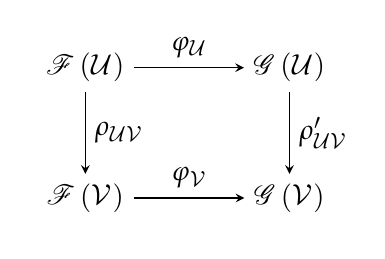
\begin{tikzpicture}
		\matrix (m) [matrix of math nodes,row sep=3em,column sep=4em,minimum width=2em]
		{
			\mathscr F\left( \sU\right)   & \mathscr G\left( \sU\right)\\
			\mathscr F\left( \sV\right)    & \mathscr G\left( \sV\right)\\
		};
		\path[-stealth]
		(m-1-1) edge node [above] {$\varphi_\sU$} (m-1-2)
		(m-1-1) edge node [right] {$\rho_{\sU\sV}$} (m-2-1)
		(m-1-2) edge node [right] {$\rho'_{\sU\sV}$} (m-2-2)
		(m-2-1) edge node [above] {$\varphi_\sV$} (m-2-2);
	\end{tikzpicture}
	\\
	is commutative, where $\rho_{\sU\sV}$ and $\rho'_{\sU\sV}$ are the restriction maps in $\mathscr F$  and $\mathscr G$. If $\mathscr F$  and $\mathscr G$ are sheaves on $\sX$, we use the same definition for a morphism 
	of sheaves. An isomorphism is a morphism  which has a two-sided inverse. 
\end{definition}

\begin{prdf}\label{sheaf_prdf}\cite{hartshorne:ag}
	Given a presheaf $\mathscr F$, there is a sheaf  $\mathscr F^+$ and a morphism $\th: \mathscr F \to \mathscr F^+$, with the property that for any sheaf  $\mathscr G$, and any morphism $\varphi: \mathscr F \to \mathscr G$, there is a unique morphism $\psi:\mathscr F^+\to \mathscr G$ such that $\varphi = \psi \circ \th$. Furthermore the pair $\left(\mathscr F^+, \th\right)$ is unique up to unique isomorphism. $\mathscr F^+$ is called the $\mathrm{sheaf~associated}$ to the presheaf $\mathscr F$. 
\end{prdf}

\begin{empt}\label{sheaf_empt}
	Following text is the citation of the proof of \ref{sheaf_prdf} (cf. \cite{hartshorne:ag}). For any open set $\sU$, let $\mathscr F^+\left(\sU\right)$ be set of functions $s$ from $\sU$ to the union $\bigcup_{x \in \sU}  \mathscr F_x$ of stalks of $\mathscr F$ over points of $\sU$, such that
	\begin{itemize}
		\item [(1)] for each $x \in \sU$, $s\left(x\right)\in \mathscr F_x$, and
		\item[(2)] for each $x \in \sU$, there is a neighbourhood $\sV$ of $x$ contained in $\sU$ and an element $t \in \mathscr F\left(\sV\right)$, such that for all $y \in \sV$ the stalk (germ) $t_y$ of $t$ at $y$ is equal to $s\left(y\right)$.
	\end{itemize}
\end{empt}
\begin{definition}\label{constant_presheaf_defn}\cite{johnstone:topos}
	If $F$ is a set and $\sX$ is a topological space then the $F$-\textit{constant presheaf} is given by
	\bean
	\sU \mapsto F.
	\eean
The $F$-\textit{locally constant sheaf} is the sheaf associated with the $F$-{constant presheaf}. We denote it by
\be
\overline{F} \bydef \text{ the sheaf associated with } F-\text{locally constant sheaf}.
\ee
\end{definition}



\begin{definition}\label{sheaf_inv_im_defn}\cite{hartshorne:ag}
	Let $f: \sX\to \sY$ be a continuous map of topological spaces. For any sheaf  $\mathscr F$ on $\sX$, we define the \textit{direct image} sheaf  $f_*\mathscr F$ on $\sY$ by $\left(f_*\mathscr F\right)\left(\sV\right)= \mathscr F\left(f^{-1}\left(\sV\right)\right)$ for any open set $\sV \subseteq \sY$. For any sheaf  $\mathscr G$ on $\sY$, we define the \textit{inverse image} sheaf  $f^{-1}\mathscr G$ on $\sX$ be the sheaf  associated to the presheaf  $\sU \mapsto \lim_{\sV \supseteq f\left(\sU\right)} \mathscr G\left(\sV\right)$, where $\sU$ is any open set in $\sX$, and the limit is taken over  all open sets $\sV$ of $\sV$ containing $f\left(\sU\right)$.
\end{definition}
%\begin{definition}\label{flabby_sheaf_defn}\label{bredon:sheaf}
%5.1. Definition. 
%A sheaf $\mathscr A$ on $\sX$ is \textit{flabby} or \textit{flasque} if $\mathscr A\left( \sX\right) \to \mathscr A\left( \sU\right)$ is surjective for every open set  $\sU \subset \sX$
%\end{definition}
\begin{proposition}\label{sheaf_flasque_prop}\cite{hartshorne:ag}
	%Proposition 2.5. // 
	If $\mathscr F$ is a flasque sheaf on a topological space $\sX$, then  $H^p\left(\sX, \mathscr F \right)  = 0$ for all $p > 0$.
\end{proposition}
\begin{definition}\label{sheaf_support_defn}
	For $s \in \mathscr{F}\left(\sX \right)$, 
	\be\label{sheaf_supp_eqn}
	\left|  s\right| = \left\{\left.x \in \sX \right|s\left(x \right)\neq 0  \right\}
	\ee
	denotes the \textit{support} of the section $s$.
\end{definition}	

If  $\dim \H = \infty$ and $\left\{L_0, L_1, ...\right\}$ is a set of mutually orthogonal codimension one projective subspaces of $\C P\left(\H \right)$ then
$$
\C P\left( \H\right) = \bigcup_{j=0}^\infty \left( \C P\left(\H \right) \setminus L_j\right) 
$$
Similarly 
$$
\C P^n = \bigcup_{j=0}^{n} \left( \C P^n \setminus L_j\right). 
$$
where $\left\{L_0,  ..., L_n\right\}$ is a set of mutually orthogonal codimension one projective subspaces of $\C P^n$.
\begin{definition}\label{nerve_defn}\cite{spanier:at}
	Given a set $X$ and a collection $\mathscr W = \left\{W\right\}$ of subsets of $X$, the \textit{nerve} of $\mathscr W$ denoted by $K\left( \mathscr W\right)$, is  the simplicial complex whose simplexes are finite nonempty subsets of  $\mathscr W$ with nonempty intersections. Thus the vertices of $K\left( \mathscr W\right)$ are nonempty elements of $\mathscr W$.
\end{definition}
\begin{theorem}\label{top_nerve_thm}\cite{bredon:sheaf}
	%PAGE 193 !!! DOWN !!!
	%4.13. Theorem. 
	Let $\mathscr A$ be a sheaf of Abelian groups  on $\sX$ and let $\mathscr U = \left\{\sU_\a\right\}_{\a \in I}$ an open covering  of $\sX$ having the property that $H^p\left( \sU_{\sigma};\mathscr A \right)= 0$  for $p > 0$ and
	all $\sigma \in K\left(\mathscr U \right)$ in the nerve of covering (cf. Definition \ref{nerve_defn}). Then there is a canonical isomorphism
	\be
	H^*\left(\sX, \mathscr A \right) \cong \check H^*\left( \mathscr U; \mathscr A\right). 
	\ee
\end{theorem}
If $\mathscr W= \left\{ \C P\left(\H \right) \setminus L_j\right\}_{j = 0, 1, ... }$ or  $\mathscr W= \left\{ \C P^n\setminus L_j\right\}_{j = 0,..., n }$ then
\be\label{nerve_eqn}
\begin{split}
	\forall \sigma \in K\left(\mathscr W\right)\quad \sU_{\sigma} = \sH \setminus \bigcup_{j = 0}^{n_\sigma} L^\sigma_j,\\
	\forall j = 1,..., n \quad L^\sigma_j \text{ is a linear subspace of } \sH \quad \codim_{\R} ~ L^\sigma_j  \ge 2,
\end{split}
\ee
From the equation \eqref{nerve_eqn} it follows that 
\be\label{nerve_0_eqn}
\begin{split}
	\mathfrak{Lattice}\left(\sU_{\sigma} \right) \cong \mathfrak{Lattice}\left(\H' \right),\\
	\forall p > 0 \quad \forall \sigma \in K\left(\mathscr W\right) \quad H^p\left( \sU_{\sigma};\mathscr A \right)= 0.
\end{split}
\ee
where $\sH'$ is a Hilbert space and the isomorphism of semi-lattices comes from the inclusion 
$\sU_{\sigma}\subset \sH'$.
If  $F$ is an Abelian group and  $\overline F$ is  $F$-locally constant sheaf  (cf, Definition \ref{constant_presheaf_defn}) on $\C P\left(\H \right)_{\mathfrak{Hausdorff}}$ (cf, Definition  and $\mathscr W= \left\{ \C P\left(\H \right) \setminus L_j\right\}_{j = 0, 1, ... }$ or  $\mathscr W= \left\{ \C P^n\setminus L_j\right\}_{j = 0,..., n }$ then 
$H^p\left( \sU_{\sigma};\mathscr A \right)= 0$  for $p > 0$ and
all $\sigma \in K\left(\mathscr W\right)$ where  $K\left(\mathscr W\right)$ is the nerve of $\mathscr W$ (cf. Definition \ref{nerve_defn}). 

\begin{theorem}\label{compact_thm}
For any Abelian group $F$ the map $\phi_{\H} : \C P\left(\H \right)_{\mathfrak{Hausdorff}}\to \C P\left(\H \right)_{\mathfrak{Gelfand}}$ yields  the natural isomorphism
$$
\mathfrak{Gelfand}\left(\K\left(\H \right) \right)\cong H^*\left(\C P\left(\H \right) _{\mathfrak{Gelfand}}, \overline F \right) \cong H^*\left(\C P\left(\H \right) _{\mathfrak{Hausdorff}}, \overline F\right)
$$
where $\overline F$ is the $F$-locally constant sheaf (cf. Definition \ref{constant_presheaf_defn}).

\end{theorem}
\begin{proof}
	If $\mathscr W$ is given by \eqref{nerve_eqn} then from the equation \eqref{nerve_0_eqn} and the Theorem \ref{top_nerve_thm} it follows that
$$
H^*\left(\C P^n_{\mathfrak{Hausdorff}}, \overline F \right) \cong \check H^*\left( \mathscr W; \overline F\right).
$$

Taking into account that $\C P^n \setminus L_j$ is open in $\C P\left(\H \right)_{\mathfrak{Gelfand}}$ for any $j$ one has
\be\label{proj_h_eqn}
H^*\left(\C P\left(\H \right) _{\mathfrak{Gelfand}}, \overline F \right) \cong H^*\left(\C P\left(\H \right) _{\mathfrak{Hausdorff}}, \overline F\right)
\ee
\end{proof}
\begin{remark}
The spectrum of $\K\left(\H \right)$ has the single point but cohomology of $\mathfrak{Gelfand}\left(\K\left(\H \right)  \right)$ are not trivial. 
\end{remark}
%\begin{definition}\label{top_paracompact_defn}\cite{munkres:topology}
%	A space $\sX$ is \textit{paracompact} if every open covering $\sX = \cup~\sU_{   \a}$ has a locally finite open refinement $\sX = \cup~\sV_{   \bt}$.
%\end{definition}	
%	\begin{lemma}\label{cw_p_lem}\cite{miyazaki_cw}
%	Any $CW$-complex is paracompact.
%\end{lemma}
\subsection{Hausdorff blowing-up}
	
	\begin{definition}\label{blowing_defn}
	If $A$ is a $C^*$-algebra then an inclusion $\mathfrak {Blowing}_{\sX-A }:C_0\left( \sX\right) \hookto M\left(A \right)$  (or equivalently $C_0\left( \sX\right) \subset M\left(A \right)$ ) is \textit{Hausdorff blowing-up} of $A$ if  both sets
		\be\label{blowing_eqn}
		\begin{split}
			C_c\left( \sX\right)A \bydef \left\{fa| f \in C_c\left( \sX\right)\quad a \in A \right\},\\
			AC_c\left( \sX\right) \bydef \left\{af| f \in C_c\left( \sX\right)\quad a \in A \right\}
		\end{split}
		\ee
		are dense in $A$.
	\end{definition}
	
	\begin{remark}\label{blowing_rem}
		$C_c\left( \sX\right)A$ is dense in $A$ if and only if $AC_c\left( \sX\right)$ is dense in $A$ (cf. equations \eqref{blowing_eqn}), i.e. both equations \eqref{blowing_eqn} are equivalent.
	\end{remark}
	
	
	
	%\begin{empt}\label{blowing_k_theory_empt}
	%	If $A$ be is  stable $C^*$-algebra then $A \cong \K\otimes A\cong A\otimes \K$. Moreover  if  $C_0\left( \sY\right) \subset M\left( A\right)$ be Hausdorff blowing-up then one has a  natural action 
	%	\bean
	%	C_0\left(\sY \right)\times  \left(A\otimes \K \right)\to A\otimes \K
	%	% \left(\K\otimes A\right)\times C_0\left(\sY \right)\to A\otimes \K 
	%	\eean 
	%	Using it one can one can construct an  injective $*$-homomorphism  !!!
	%	$$
	%	\left(C_0\left(\sY \right) \otimes \K \right) \to A
	%	$$
	%	This homomorphism yields homomorphisms of $K$-theory
	%	\bea\label{blowing_k0_eqn}
	%	K^0\left(\sY \right)\cong K_0\left(C_0\left( \sY\right)  \right) \to K_0\left( A\right),\\\label{blowing_k1_eqn}
	%	K^1\left(\sY \right)\cong K_1\left(C_0\left( \sY\right)  \right) \to K_1\left( A\right).
	%	\eea 
	%	If $A$ is an  irrational rotation algebra of torus then the map $K_1\left(C_0\left( \sY\right)  \right) \to K_1\left( A\right)$ is an isomorphism.
	%\end{empt}
	%\begin{example}\label{blowing_hausdorff_exm}	If $A$ is a  given by \eqref{cross_mult_eqn} $C^*$-algebra with Hausdorff spectrum $\sX$  then from the Theorems \ref{oa_haus_prim_thm} and  \ref{dauns_hofmann_thm} one has the natural inclusion $C_0\left(\sX \right) \hookto M\left( A\right)$, which is Hausdorff blowing-up.
	%\end{example}
	
	\begin{definition}\label{blowing_ideals_au_ua_defn}
		Let  $ C_0\left( \sX\right)\subset  M\left( A\right) $ be  Hausdorff blowing-up of $A$ (cf. Definition \ref{blowing_defn}), and let $\sU \subset \sX$ be an open subset. Both   left and right  closed ideals $A_\sU$  and $_\sU A$ of $A$ generated by sets 	$AC_0\left( \sU\right)$ and $C_0\left( \sU\right)A$ are the \textit{left} $\sU$-\textit{ideal} and the \textit{right} $\sU$-\textit{ideal} respectively. A hereditary $C^*$-subalgebra of $A$
		\be\label{blowing_hereditary_u_eqn} 
		\begin{split}
			_\sU A_\sU \bydef	~	_\sU A\cap  A_\sU = A^*	_\sU \cap  A_\sU\\ %(\text{cf. Definition \ref{hered_defn} and the Lemma \ref{hered_bab_lem}}).
		\end{split}
		\ee	
		is the $ \sU$-\textit{subalgebra}.
		
	\end{definition}
	
	
	\begin{lemma}\label{blowing_compact_lem}
		If $C\cong C_0\left( \sY\right) \subset M\left(A \right)$ is    {Hausdorff blowing-up} of $A$  (cf. Definition \ref{blowing_defn}	for any $a \in A$ and $\eps > 0$ following conditions hold:
		\begin{enumerate}
			\item[(i)] there is a positive $f \in C_c\left( \sY\right)_+$ with 
			\be\label{blowing_compact_eqn}
			\begin{split}
				\left\| f  \right\| \le 1,\\
				\left\| a - af  \right\|< \eps,\\
				\left\| a - fa \right\|< \eps,\\
				\left\| a - faf  \right\|< \eps,
			\end{split}
			\ee
			\item[(ii)] there are an open subset $\sU \subset \sY$ with compact closure and $b \in ~_\sU A_\sU$ such that
			\be\label{blowing_compact_b_eqn}
			\begin{split}
				b \in  ~_\sU A_\sU,\\
				\left\| a - b \right\|< \eps.
			\end{split}
			\ee
		\end{enumerate}
	\end{lemma}
	\begin{proof}(i)
		If $g \in C_c\left( \sY\right)$ then $g = fg = gf$ for any positive $f \in C_c\left( \sY\right)_+$ such that
		\bean
		\left\| f \right\|= 1,\\
		f\left(\supp g \right) = 1.
		\eean 
		If $f' \in C_c\left( \sY\right)$ and $c' \in A$ such that
		$\left\|a-f'c' \right\| < \eps/4$ (cf. equation \eqref{blowing_eqn}) then there for any positive $f_1$ such that $\left\| f_1 \right\|= 1$, $~f_1\left(\supp f' \right) = 1$ one has
		\bean
		\left\|f_1\left( a-f'c \right) \right\|\le \left\|f_1 \right\|\left\|a-f'c \right\|\le \frac{\eps}{4},\\
		\left\|a-f_1a \right\| < \left\|f_1a - f_1f'c\right\|+ \left\|a - f_1f'c\right\|\le \frac{\eps}{2}
		\eean
		Similarly 	If $f'' \in C_c\left( \sY\right)$ and $c''/ \in A$ such that
		$\left\|a-f'c'' \right\| < \eps/4$ then for any positive for any positive $f_2$ such that $\left\| f_2 \right\|= 1$, $~f_1\left(\supp f' \right) = 1$ one has
		\bean
		\left\|a-a f_2 \right\| <  \frac{\eps}{2}
		\eean
		If $f = \max\left(f_1, f_2 \right)$ then $f\left(\supp f' \cup \supp f'' \right)= \{1\}$ 
		and
		\bean
		\begin{split}
			\left\| f  \right\| \le 1,\\
			\left\| a - af  \right\|< \frac{\eps}{2},\\
			\left\| a - fa \right\|< \frac{\eps}{2},\\
		\end{split}
		\eean
		On the other hand
		\bean
		\left\| a - faf \right\|\le \left\| a - fa \right\|+ \left\| fa - faf \right\|< \frac{\eps}{2}+ 	\left\| f\right\|\left\|a - fa\right\|< \eps.
		\eean
		(ii) The set $\sU \bydef \left\{y \in \sY | f\left(y\right)\neq 0\right\}\subset \sY$ is open and closure of $\sU$ is the compact set $\supp f$. Moreover  $f a f \in ~_\sU A_\sU$ and  $\left\|a - faf\right\|< \eps$.
		
	\end{proof}
	%\begin{empt}\label{blowing_compact_supp_empt}
	%	If $\left\{\sU_\la\right\}_{\la\in\La}$ is a given by the Corollary	\ref{top_connected_union_cor} family of open subsets of $\sY$ with compact closures then $\sY = \cup_{\la \in \La} \sU_\la$. Since the family is directed the union $A_c \bydef \cup_{\la \in \La} \sU_\la$ is a $*$-subalgebra of $A$. From the Lemma \ref{blowing_compact_lem} it follows that $A_c$ is dense in $A$.
	%\end{empt}
	%\begin{definition}\label{blowing_compact_supp_defn}
	%	The given by \ref{blowing_compact_supp_empt} dense $*$-subalgebra $A_c \subset A$ is said to be the \textit{algebra of compactly supported elements}.
	%\end{definition}
	
	
	\begin{empt} 
		
		We leave to the reader a proof of following equations:
		\be\label{blowing_su_eqn}
		\begin{split}
			_\sU A \bydef \left\{ a \in A~ |~ \forall f \in C_0\left( \sY\right)\quad f\left(\sU \right)= \{0\}  \quad \Rightarrow \quad fa = 0\right\} ,\\
			A_\sU \bydef \left\{ a \in A~ |~ \forall f \in C_0\left( \sY\right)\quad  f\left(\sU \right)= \{0\} \quad \Rightarrow \quad af = 0\right\}
		\end{split}
		\ee
		
		
		\bea\label{blowing_sue1_eqn}
		\sU'\cap \sU'' =\emptyset\quad \Rightarrow\quad A_{\sU'}~_{\sU''}A= \{0\}.
		\eea
		
		From \eqref{blowing_su_eqn} it follows that
		\be\label{blowing_su_inc_eqn}
		\sU'\subset \sU'' \quad \Rightarrow\quad _{\sU'}A \subset~  _{\sU''}A ~\text{ AND } ~A_{\sU'}\subset A_{\sU''}~\text{ AND }~  _{\sU'}A _{\sU'}\subset _{\sU''}A _{\sU''}.
		\ee
	\end{empt}
	
	\begin{definition}\label{blowing_support_defn}
		If $C_0\left( \sX\right) \subset M\left(A \right)$ is    {Hausdorff blowing-up} of $A$  (cf. Definition \ref{blowing_defn}),  $a \in A$ and
		$
		\sU_a \bydef\bigcap 
		\left\{\left.{\sU} \subset \sX\right| a\in~_\sU A_{\sU} \right\}
		$
		then the  closure $\sV_a$  of $\sU_a$ is said to be the \textit{support} of $a$. We write $\supp a \bydef \sV_a$.
	\end{definition}
	
	\begin{lemma}\label{pedersen_eps_lem}
		Let $\eps > 0$, and let 	 $f_\eps: \R \to \R$ be a continuous function given by 
		\begin{equation}\label{f_eps_eqn}
			f_\eps\left( x\right)  \bydef\left\{
			\begin{array}{c l}
				0 &x \le \eps \\
				x - \eps & x > \eps
			\end{array}\right.
		\end{equation}
		If $A$ is a $C^*$-algebra 
		then one has
		\bea\label{k0_ped_e_eqn}
		K\left( A \right)_0 = \left\{f_\eps \left(a\right) \left|~a \in A_+, \quad \eps > 0 \right.\right\},~~~\\
		\label{kp_ped_e_eqn}
		K\left( A \right)_+ = \left\{a \in A_+ \left|a \le \sum_{j = 1}^n f_{\eps_j}\left(  a_j\right) \quad a_j \in  	K\left( A \right)_0\quad \eps_j > 0\quad j=1,...,n\right.\right\}~~
		\eea
		where both $	K\left( A \right)_0$ and 	$K\left( A \right)_+$ are given by equations \eqref{pedersen_k0_eqn} and \eqref{pedersen_k_plus_eqn} respectively
	\end{lemma}
	\begin{proof}
		If  $a\in A_+$ and $\eps > 0$ then $f_\eps \left(a\right)= \phi_\eps\left(a \right)$ where  $\phi_\eps \in K(]0, \infty [$ is given by 
		\bean
		\phi_\eps\left( x\right)  =\left\{
		\begin{array}{c l}
			0 &x \le \eps \\
			x - \eps &  \eps \le x \le \left\| a\right\|\\
			2	\left\| a\right\| - \eps - x & \left\| a\right\| \le x \le 2\left\| a\right\|-\eps\\
			0 & x \ge 2 \left\| a\right\| -\eps\\
		\end{array}\right.
		\eean
		It follows that $f_\eps\left(a\right)	\in K\left( A \right)_0$. Conversely  if $a \in	K\left( A \right)_0$ then from \eqref{pedersen_k0_eqn} it turns out that there is $b \in A_+$ and $\varphi \in   K(]0, \infty [$ such that $a = \varphi\left(b\right)$. If  $\supp \varphi \subset \left[\eps, c\right]$ and  $\psi \in C_c\left( \R\right)_+$ is given by
		\bean
		\psi\left( x\right)  =\left\{
		\begin{array}{c l}
			0 &x \le 0 \\
			x &0 \le x \le \eps \\
			\varphi\left(x\right) + \eps &\eps \le x \le c \\
			\eps + c - x&  c \le x \le c+ \eps\\
			0 & x \ge c + \eps
		\end{array}\right.
		\eean
		then $ \varphi = f_\eps  \circ\psi$. It follows that $a = f_\eps\left(b' \right)$ where $b' \bydef \psi\left(b\right)$. So the equation \eqref{k0_ped_e_eqn} is proven. The equation \eqref{kp_ped_e_eqn} is a direct consequence of \eqref{k0_ped_e_eqn} and \eqref{pedersen_k_plus_eqn} ones.
		
	\end{proof}
	
	
	
	
	
	\begin{lemma}\label{blowing_pedersen_compact_lem}
		If  $C_0\left( \sX\right)\hookto M\left( A\right)$ is Hausdorff blowing-up and $a\in A$ belongs to the Pedersen's ideal $K\left(A \right)$ (cf. Definition \ref{pedersen_ideal_defn}) then the support of $a$ (cf. Definition \ref{blowing_support_defn}) is compact.
	\end{lemma}
	\begin{proof}
		If $a \in K\left(A\right)_0$ (cf \eqref{pedersen_k0_eqn}) then from the Lemma  \eqref{pedersen_eps_lem} it follows that there is $\eps > 0$ and $b \in A_+$ such that $a = f_\eps \left( b\right)$ where $f_\eps$ is given by \eqref{f_eps_eqn}. On the other hand  there is a positive element   $c\in  A_+$  such that $\left\|c - b \right\|  < \eps/2$ and $\supp c$ is compact (cf. Definition  \ref{blowing_defn}).
		If $a \le c$ does not hold and $\rho: A \hookto B\left(\H \right)$ is a faithful  nondegenerate representation  then there is $\xi \in \H$ such that
		\bean\label{blowing_ac_eqn}
		\forall \xi \in \H \quad \left( \xi, \rho\left( a \right) \xi\right) > \left( \xi, \rho\left( c \right) \xi\right)
		\eean
		From $\left\|c - b \right\|  < \eps/2$ if follows that
		\be\label{blowing_acc_eqn}
		\forall \xi \in \H  \quad \left\| \xi \right\| = 1\quad \Rightarrow\quad  \left|\left( \xi, \rho\left( b \right) \xi\right)-\left( \xi, \rho\left( c \right) \xi\right) \right| < \eps/2
		\ee
		On the other hand from $a =f_\eps \left( b\right)> 0$ it follows that there is $\xi \in \H$ and $\la \in \R_+$ such that
		\bean
		\left\| \xi \right\| = 1,\\
		\rho\left(a \right) \xi = \la \xi,\\
		\rho\left(b \right)\xi = \left( \la+\eps \right) \xi,\\
		\rho\left(a \right)\xi = \la  \xi,\\
		\left( \xi, \rho\left( b \right) \xi\right) - \left( \xi, \rho\left( a \right) \xi\right)= \eps
		\eean
		and taking into account \eqref{blowing_acc_eqn} one has
		$$
		\left( \xi, \rho\left( c \right) \xi\right)- \left( \xi, \rho\left( a \right) \xi\right)> \frac{\eps}{2}
		$$
		Above condition contradicts with \eqref{blowing_ac_eqn} so $a \le c$.
		If $\supp a \subsetneqq \supp c$ then there is a nonempty  open set  $\sU \subset \supp a\setminus \supp c$. For any $f \in C_0\left(\sU \right)\setminus \{0\}$ one has
		\bean
		faf^* > 0,\\
		fcf^* = 0.
		\eean
		However it is impossible since $a \le c$, so $\supp a \subsetneqq \supp c$ is not true and $\supp a \subset\supp c$. Thus the set $\supp a$ is a closed subset of the compact set $\supp c$ therefore $\supp a$ is compact. Using this fact and the Definition \ref{pedersen_ideal_defn} we conclude that $\supp a$ is compact for any $a \in K\left( A\right)$. 
	\end{proof}
	\begin{remark}
		The Lemma \ref{blowing_pedersen_compact_lem} can be regarded as a generalization of the equation  \eqref{peder_c0_eqn}.
	\end{remark}
	
	\begin{proposition}\label{spectral_sequence_prop}\cite{johnstone:topos}
		%8.17 
		Let $\sX \xrightarrow{f} \sY$ be a continuous map then
		\begin{enumerate}		\item [(i)] 
			if $\mathscr A$ is sheaf of  Abelian group in $\sY$ then we have a homomorphism $H^q\left(\sY, \mathscr A \right) \xrightarrow{} H^q \left(\sX, f^*\mathscr A\right)$ for each $q$ which is functorial in $f$ and natural in $\mathscr A$.
			\item [(ii)] If $\mathscr B$ is a sheaf of Abelian groups in $\sX$ then we have a spectral sequence (Leray spectral sequence) $H^p\left(\mathscr \sY, R^qf_*\left(\mathscr B \right) \right)\Rightarrow H^{p + q}\left(\sX, \mathscr B \right)$ which is natural in $ \mathscr B$.
		\end{enumerate}
	\end{proposition}
	\begin{remark}
		The above formulation of the Proposition \ref{spectral_sequence_prop} differs from the described in \cite{johnstone:topos} more general one.
	\end{remark}
		\begin{remark}\label{blow_rem}
	From the equation  \eqref{peder_c0_eqn} it follows that the injective homomorphism $\varphi_\sX : C_0\left(\sX \right) \hookto M\left(A \right)$ is good (cf. Definition \ref{good_defn}). So there is the natural surjective continuous map
	\be\label{phi_a_eqn}
	\phi_A : \mathfrak{Gelfand}\left(A \right) \to \sX.
	\ee
	\end{remark}
	\begin{empt}

%\begin{theorem}\label{loc_fin_french_thm}\cite{godement:sheaf}
	%Th�or?me 1.3.1.�? 
%	Soient $\mathscr F$ un faisceau de base $\sX$ et $\left\{M_\iota\right\}_{\iota\in I}$ un recouvrement 	ferm� localement fini de $\sX$. Supposons donn�es des sections $s_\iota \in \mathscr F\left(M_\iota \right)$  de telle sorte que 	$s_\iota = s_j$ dans $M_\iota \cap M_j$- quels que soient $\iota$ et $j$; alors il existe une section  $s \in \mathscr F\left(\sX \right)$ qui 	co\"incide avec $s_\iota$ dans $M_\iota$- quel que soit $\iota \in I$. 
%\end{theorem}
%Following theorem is an English translation of the \ref{loc_fin_french_thm} one.
%\begin{theorem}\label{loc_fin_eng_thm}\cite{godement:sheaf}
%	Let $\sX$ is a topological space, and let $\mathscr F \in \mathbf{Sh}\left( \sX\right)$. Let $\left\{M_\iota\right\}$ is a locally finite closed covering of $\sX$, and let $s_\iota \in \mathscr F\left( M_\iota \right)$ be such that $s_\iota = s_j$ on $M_\iota \cap M_j$ for all $\iota$ and $j$. Then there is $s \in \mathscr F\left( \sX\right)$ 
%\end{theorem}
%\begin{theorem}\label{closed_cov_thm}\cite{godement:sheaf}
%	Let $\mathscr U$ be either open covering or locally finite closed covering of $\sX$. For any sheaf $\mathscr A$ there is a canonical isomorphism
%	$$
%	H^0\left(\mathscr U; \mathscr A \right) \cong \Ga\left(\mathscr A \right)\cong H^0\left(\sX; \mathscr A \right).
%	$$
%\end{theorem}	
	If $C_0\left(\sY \right) \xrightarrow{f} M\left(A \right)$ is Hausdorff blowing-up then 
from the Remark \ref{blow_rem} and the Proposition \ref{spectral_sequence_prop} it follows that
\begin{enumerate}	
		\item [(i)] 
	if $\mathscr A$ is sheaf of  Abelian group in $\sY$ then we have a homomorphism $H^q\left(\sY, \mathscr A \right) \xrightarrow{} H^q \left(\mathfrak{Gelfand}\left(A \right) , \phi_A^*\mathscr A\right)$ for each $q$ which is functorial in $f$ and natural in $\mathscr A$.
	\item [(ii)] If $\mathscr B$ is a sheaf of Abelian groups in $\sX$ then we have a spectral sequence (Leray spectral sequence) $H^p\left(\mathfrak{Gelfand}\left( A\right) , R^q\left(\phi_A \right) _*\left(\mathscr B \right) \right)\Rightarrow H^{p + q}\left(\sX, \mathscr B \right)$ which is natural in $ \mathscr B$.
\end{enumerate}
\end{empt}
\begin{empt}\label{blowing_empt}
	Let $A$ be a $C^*$-algebra with the spectrum $\sY$ such that
	\be\label{norm_eqn}
	\forall a \in A\quad \left\|a \right\| = \sup_{y \in \sY} \left\| \rho_y\left(a \right) \right\| 
	\ee
where $\rho_y: A \to B\left(\H_y \right)$ is the corresponding to $y$ irreducible representation. 
\end{empt}

\begin{lemma}\label{hausdorff_spectrum_lem}\cite{rae:ctr_morita}
	Suppose $A$ is a $C^*$-algebra with Hausdorff spectrum $\mathcal{X}$.
	\begin{itemize}
		\item [(a)] If $a, b \in A$ and $\mathfrak{rep}_x\left(a \right)=  \mathfrak{rep}_x\left(b \right)$ for every $x \in  \mathcal{X}$, then $a = b$.
		\item[(b)] For each $a \in A$ the function $x \mapsto \left\|\mathfrak{rep}_x\left(a \right) \right\|$ is continuous on  $\mathcal{X}$, vanishes at infinity and has sup-norm equal to $\left\| a\right\|$. 
	\end{itemize}
\end{lemma}

\begin{remark}
	It is known that following $C^*$-algebra satisfy to the condition \eqref{norm_eqn}.
	\begin{itemize}
		\item Any $C^*$-algebra  with Hausdorff spectrum (cf. Lemma \ref{hausdorff_spectrum_lem}).
		\item Any reduced $C^*$-algebra of foliation (cf, \cite{candel:foliII}).
	\end{itemize}
\end{remark}
\begin{empt}

If $C^*$-algebra $A$ satisfies to \eqref{norm_eqn}, $\sY$ is the spectrum of $A$ and $S\subsetneqq A$ is a closed subset then there is $a \in A\setminus S$ and $\eps > 0$ such that
$$
\forall a' \in S\quad  \left\| a - a' \right\| > 2\eps
$$
It turns out that there is $y \in \sY$ such that
$$
\forall a' \in S\quad  \left\| \rho_y\left(a - a' \right) \right\| > \eps
$$
If $L\subset A$ is a proper closed left ideal then there is $y \in \sY$ such that
\be\label{to_sp_eqn}
\rho_y\left( L\right) \H_y \neq \H_y.
\ee
If for all  $\xi \in \mathfrak{Gelfand}\left(A \right)$  such that there is a bicommutant (cf, Definition \ref{bicommutant_defn}) $\xi'' \subset A$ then there is the unique $y \in \sY$ such that $\rho_y\left( L\right) \H_y \neq \H_y$. It turns out that there are following maps
\be\label{gg_m_eqn}
\begin{split}
\mathfrak{Gelfand}\left(A \right) \to \mathfrak{Gelfand}\left(A \right)'' \to \sY.
\end{split}
\ee
The maps \ref{gg_m_eqn} are specializations of \eqref{to_sp_eqn} ones.
If there is a map $\sX \xrightarrow{\mathfrak{Blowing}} \sY$ such that the following diagram commutative 
	\newline
\begin{tikzcd}
	\mathfrak{Gelfand}\left( A\right)	 \arrow[rr, "\phi_A"]\arrow[rd]  & ~ & \sX \arrow[ld, , "\mathfrak{Blowing}"]\\
	& \sY &
\end{tikzcd}
\\
then $\mathfrak{Blowing}$ is said to be \textit{blowing - up}.
\end{empt}
\begin{example}\label{foli_exm}
The notions of foliation and its $C^*$-algebra are explained in \cite{candel:foliI,candel:foliII}. A foliated manifold $\left(M, \F \right)$ contains a differential manifold $M$ such that
$$
M = \bigsqcup_{\la \in \La} \L_\la
$$
where $\L_\la$ is a set of leaves. If any leaf simply connected then any irreducible representation correspond to a leaf. There is an equivalence relation on $M$ such that
$$
x' \sim x'' \quad \exists \la\in \La \quad x', x'' \in \L_\la
$$ 
It is proven that the spectrum of the explained in \cite{candel:foliII} reduced $C^*$-algebra of 	$C^*_r\left(M, \F \right)$ naturally homeomorphic to $M/ \sim$. Otherwise there is Hausdorff blowing-up $C_0\left( M\right) \to M\left(C^*_r\left(M, \F \right) \right)$. In result one has the following diagram
	\newline
\begin{tikzcd}
	\mathfrak{Gelfand}\left(C^*_r\left(M, \F \right)\right)	 \arrow[rr, "\phi_{(C^*_r\left(M, \F \right)}"]\arrow[rd]  & ~ & M \arrow[ld, , "\mathfrak{Blowing}"]\\
	& M/\sim &
\end{tikzcd}
\\
  
\end{example}

\begin{remark}
then we say that $\mathfrak{Blowing}$ is the Hausdorff blowing-up of the spectrum.
The "blowing-up" word is inspired by following reasons:
\begin{itemize}
	\item the existence  of the  surjective  map $\mathfrak{Blowing}$ from the  Hausdorff space  to the spectrum, %(cf. Definition \ref{blowing_spectral_defn}),
	\item  in the algebraic geometry   "blowing-up" means  from a map $\sX \to \sY$ such that the variety $\sX$ has no singular points (cf. \cite{hartshorne:ag}).
\end{itemize}
\end{remark}






\subsection{Gelfand space of continuous trace $C^*$-algebra}
\subsubsection{Basic construction}

\begin{definition}\label{abelian_element_defn}\cite{pedersen:ca_aut}
	A positive element in $C^*$ - algebra $A$ is {\it Abelian} if subalgebra $xAx \subset A$ is commutative.
\end{definition}
\begin{definition}\label{continuous_trace_c_alt_defn}\cite{rae:ctr_morita}
	%Definition 5.13. 
	A \textit{continuous-trace} $C^*$-\textit{algebra} is a $C^*$-algebra $A$ with Hausdorff
	spectrum $\sX$ such that, for each $x_0\in\sX$ there are a neighbourhood $\sU$ of $x_0$ and $a\in A$ such that $\rep_{ x}\left( a\right) $ is a rank-one projection for all $x \in \sU$.
\end{definition}
	\begin{thm}(Dauns Hofmann)\label{dauns_hofmann_thm}\cite{pedersen:ca_aut}
	For each $C^*$-algebra $A$ there is the natural isomorphism from the center of $M\left( A\right)$ onto the class of bounded continuous  functions on $\check{A}$. 
\end{thm}

\begin{lemma}\label{ctr_g_lem}
	If  $A$ is a {continuous-trace} $C^*$-{algebra} then the  bicommutant of Gelfand space (cf. Definition \ref{bicommutant_defn}) is equivalent to the  a set of pairs $\left(x_\xi, V_\xi \right)$ where $x_\xi \in \sX$ is an element of the spectrum $\sX$ of $A$ and $V$ is a one dimensional subspace of the corresponding to $x$ Hilbert space $\H_x$ of irreducible representation $\rep_x: A \to B\left(\H_x \right)$.
\end{lemma}
\begin{proof}
From the Theorem \ref{dauns_hofmann_thm} and the Lemma \ref{hausdorff_spectrum_lem} it follows that there is Hausdorff blowing-up 
\be 
\mathfrak {Blowing}_{\sX-A }:C_0\left( \sY\right) \hookto M\left(A \right)
\ee

where $\sX$ is the spectrum of $A$.  So there are following maps 
\be\label{ctr_g_eqn}
\begin{split}
	\mathfrak{Gelfand}\left(A \right) \xrightarrow{\phi} \mathfrak{Gelfand}\left(A \right)'' \xrightarrow{\phi''} \sX.
\end{split}
\ee
If $\xi \in \mathfrak{Gelfand}\left(A \right)$,  $\xi'' \bydef \phi\left(\xi \right)  \in \mathfrak{Gelfand}\left(A \right)''$ and $x_\xi = \phi''\left( \xi''\right)$ then for any $x \neq x_\xi$ there and an open neighborhood  $\sU$ of $x$ such that $f \in C_0\left(\sX \right)$ with $ f\left(\sU \right)= {0}$ and $L \bydef f A \in \xi$. If $L^\perp$ is a commutant of $L$ (cf. Definition \ref{bicommutant_defn}) then $\rep_{x'} \left(L^\perp \right) = \rep_{x'}\left( A\right)$ where $\rep_{x}: A \to B\left( H_{x'}\right) $ is the corresponding to $x$ irreducible representation. It follows that $x_\xi$ is the unique point such that $\rep_{x_\xi} \left( \xi''\right) \neq \rep_x \left( A\right)$. Since $\rep_{x_\xi} \left( \xi''\right)\subset \rep_{x_\xi} \left( A\right)$ is a left ideal there is a vector subspace $V_\xi\subset \H$ such that $\rep_{x_\xi} \left( \xi''\right)V_\xi = \{0\}$. If dimension of $V_\xi$ exceeds 1 and $\eta \in V_\xi$ then the set
$$
\left\{ L \in \xi | \rep_x \left(L \right)\eta = \{0\} \right\} \subset \mathfrak{Lattuce}\left(A \right)
$$
generates a filter which exceeds $\xi$. It is impossible since the filter $\xi$ is an ultrafilter.


\end{proof}


	\begin{proposition}\label{top_final_prop}\cite{bourbaki_sp:gt}
	Let $\sX$ be a set, let $\left\{\sY_\iota\right\}_{\iota\in I}$ be a family of topological spaces, and for each $\iota\in I$ let $f_\iota$ be a mapping of $\sY_\iota$ into $\sX$. Let $\mathfrak{D}$ be a set of subsets $\sU$ of $\sX$ such that $f_\iota^{-1} \left(\sU \right)$ is open in $\sY_\iota$ for each $\iota \in I$; then  $\mathfrak{D}$ is a set of open sets in a topology $\mathfrak{T}$. In particular $\mathfrak{T}$ is the finest topology for which the mappings $f_\iota$ are continuous. In other words, if $g$ is mapping on $\sX$ into a topological space $\sZ$, then $g$ is continuous ($\sX$ carrying the topology $\mathfrak{T}$) if and only if each of the mappings $g\circ f_\iota$ is continuous.
\end{proposition}
\begin{definition}\label{top_final_defn}
	Under the hypotheses of Proposition \ref{top_final_prop} we say that the topology $\mathfrak{T}$ is \textit{final} (\textit{with respect to the family of maps} $\left\{f_\iota:\sY_\iota \to \sX\right\}_{\iota\in I}$).
\end{definition}

	\begin{proposition}\label{top_init_prop}\cite{bourbaki_sp:gt}
	Let $\sX$ be a set, let $\left\{\sY_\iota\right\}_{\iota \in I}$ be a family of topological spaces, and for each $\iota \in I$ let $f_\iota$ be a mapping of $\sX$ into $\sY_\iota$.  Let $\mathfrak{S}$ be the set of subsets of $\sX$ of the form $f^{-1}_\iota\left(\sU_\iota \right)$ where $\iota \in I$, $\sU_\iota$ is open in $\sY_\iota$. Let $\mathfrak B$ be the set of finite intersections of sets of $\mathfrak S$. Then $\mathfrak B$ is a base of a topology $\mathfrak T$ and in particular is the coarsest topology on $\sX$ for which the mappings $f_\iota$ are continuous. More precisely of $g$ is a mapping of topological space into $\sY$, then is continuous at a point  $z \in \sZ$ ($\sX$ carrying the topology $\mathfrak T$) if and only if for each of the functions $f_\iota\circ g$ is continuous at $z$.
\end{proposition}
\begin{definition}\label{top_init_defn}\cite{bourbaki_sp:gt}
	Under the hypotheses of Proposition \ref{top_init_prop} we say that the topology $\mathfrak{T}$ is \textit{initial} (\textit{with respect to the family of maps} $\left\{f_\iota:\sX \to \sY_\iota\right\}_{\iota\in I}$).
\end{definition}
\begin{empt}
		If   $A$  is a {continuous-trace} $C^*$-{algebra} with the spectrum $\sX$ then there is a presheaf  $\mathscr P_{\sX\text{-}A}$ of sets such that for any open $\sU \subset \sX$  one has
		\be\label{presh_eqn}
		\begin{split}
	\mathscr P_{\sX\text{-}A}\left(\sU \right) \bydef \left\{ C \subset A \text{ is commutative hereditary subalgebra} \left| C \subset ~_\sU A_\sU \text{ cf. \eqref{blowing_hereditary_u_eqn})}\right. \right\}\\
\rho_{\sU\sV} : \mathscr P_{\sX\text{-}A}\left(\sU \right)\to \mathscr P_{\sX\text{-}A}\left(\sV \right),\\
C \mapsto C \cap ~_\sV A _\sV.
		\end{split}
		\ee
\end{empt}
\begin{exercise}\label{sheaf_etale_exer}\cite{hartshorne:ag}
	%1.13. 
	\textit{
		\'Espace Etal\'e of a Presheaf}. %(This exercise is included only to establish the connection between our definition of a sheaf and another definition often found in the literature. See for example Godement [1, Ch. II, �1.2].)
	Given a presheaf $\mathscr F$ on $\sX$, we define a topological space $\mathrm{Sp\acute{e}}\left(\mathscr F \right)$ , called the \textit{
		\'espace etal\'e} of a presheaf of $\mathscr F$ as 
	follows. As a set it is the union $\mathrm{Sp\acute{e}}\left(\mathscr F \right)= \bigcup_{x\in\sX} \mathscr F_x$ of sets of germs (cf. Definition \ref{sheaf_stalk_defn}). We define a projection map 
	\be\label{pf_eqn}
	p_{\mathrm{Sp\acute{e}}\left(\mathscr F \right)}: \mathrm{Sp\acute{e}}\left(\mathscr F \right)\to \sX
	\ee
	by sending $s_x\in \mathscr F_x$ to $x$. Consider the initial with respect to the map $	p_{\mathrm{Sp\acute{e}}\left(\mathscr F \right)}$ topology (cf. Definition \ref{top_init_defn} and denote by $\mathrm{Sp\acute{e}}\left(\mathscr F \right)_{\mathfrak{Etale}}$ the corresponding topological space.
\end{exercise}
\begin{lemma}\label{ctr_gelfand_lem}
	If $A$ is a {continuous-trace} $C^*$-{algebra} then there is the natural bijective set theoretic map $\phi_{\mathscr P}:\mathfrak{Gelfand}\left( A\right) \cong \mathrm{Sp\acute{e}}\left(\mathscr P_{\sX\text{-}A} \right)$  with the following commutative diagram
	\newline
	\begin{tikzcd}
	\mathfrak{Gelfand}\left( A\right)		 \arrow[rr, "\cong"]\arrow[rd]  & ~ & \mathrm{Sp\acute{e}}\left(\mathscr P_{\sX\text{-}A} \right) \arrow[ld]\\
		& \sX &
	\end{tikzcd}
\end{lemma}	
\begin{proof} 
If $\xi \in 	\mathfrak{Gelfand}\left( A\right)$, $\xi'' \bydef \phi\left(\xi \right)$  and $x = \/ \phi''\left( \xi''\right)\in  \sX$ (cf. the equation \eqref{ctr_g_eqn}) then from the the Lemma  \ref{ctr_g_lem} it follows that there is a pair $\left(x_\xi, V_\xi \right)$ such that
$$
\xi'' = \left\{ b \in A \left| \rep_{x_\xi} \left(b^* \right)V_\xi = \{0\} \right.\right\}
$$ 
It follows that for any $L \in \xi$  one has $\rep_{x_\xi}\left(L \right) \H_{x_\xi}= V_\xi$. Let 
\bean
\mathrm{Sp\acute{e}}\left(\mathscr P_{\sX\text{-}A} \right)_x \bydef \left\{\left.\eta \in \mathrm{Sp\acute{e}}\left(\mathscr P_{\sX\text{-}A} \right)\right| 	p_{\mathrm{Sp\acute{e}}\left(\mathscr F \right)}\left(\eta \right) = x\right\},\\
\mathrm{Sp\acute{e}}\left(\mathscr P_{\sX\text{-}A} \right)_\xi =  \left\{\left.\zeta \in \mathrm{Sp\acute{e}}\left(\mathscr P_{\sX\text{-}A} \right)_x\right| \forall L \in \xi \quad  \exists  C \subset L^*L \quad \zeta = C_x  \right\}
\eean
where $C$ is a commutative $C^*$-subalgebra which represents $\zeta$ and $C_x$ is the germ of $C$ at $x$ (cf. Definition \ref{sheaf_stalk_defn}). If $\mathrm{Sp\acute{e}}\left(\mathscr P_{\sX\text{-}A} \right)_\xi$ contains more than one element and $\zeta \in \mathrm{Sp\acute{e}}\left(\mathscr P_{\sX\text{-}A} \right)_\xi$ then the  filter
\bean
\left\{L \subset A \left| \exists  C \subset L^*L \quad \zeta = C_x \right.\right\}
\eean 
exceeds $\xi$. It is impossible since $\xi$ is an ultrafilter. If $C', C''$ are two commutative $C^*$-algebras which correspond two elements $L', L'' \in \xi$ then one has
$$
\forall f \in C_0\left(\sX \right) \quad f\left(x \right)\neq 0 \quad\left(  \mathfrak {Blowing}_{\sX-A }(f) C'\right) \cap \left( \mathfrak {Blowing}_{\sX-A }(f) C''\right)  \neq \{0\}.
$$
It is possible if and only if and only if $C'_x = C''_x$, so there is the natural  map $\phi_{\mathscr P} :\mathfrak{Gelfand}\left( A\right) \cong \mathrm{Sp\acute{e}}\left(\mathscr P_{\sX\text{-}A} \right)$. On the other hand if $\zeta \in \mathrm{Sp\acute{e}}\left(\mathscr P_{\sX\text{-}A} \right)$ and 
$$
\xi \bydef \left\{ L \in A \left| \exists C \subset L^*\cap L \quad C_x = \zeta\right.\right\}
$$
then $\phi_{\mathscr P}\left(\xi \right) = \zeta$, i.e. the map $\phi_{\mathscr P}$ is bijective.
\end{proof}
Denote by $\mathrm{Sp\acute{e}}\left(\mathscr P_{\sX\text{-}A} \right)_{\mathfrak{Etale}}$ the set $\mathrm{Sp\acute{e}}\left(\mathscr P_{\sX\text{-}A} \right)$ supplied with the smallest topology such that the map $\mathrm{Sp\acute{e}}\left(\mathscr P_{\sX\text{-}A} \right)_{\mathfrak{Etale}}\to \sX$ is continuous. If $\mathrm{Sp\acute{e}}\left(\mathscr P_{\sX\text{-}A} \right)_{\mathfrak{Gelfand}}$ is the topological space such that the bijective map $\mathrm{Sp\acute{e}}\left(\mathscr P_{\sX\text{-}A} \right)_{\mathfrak{Gelfand}}\cong \mathfrak{Gelfand}\left( A\right)$ is  homeomorphism then since the map $\mathfrak{Gelfand}\left( A\right)\to \sX$ is continuous the topology of $\mathrm{Sp\acute{e}}\left(\mathscr P_{\sX\text{-}A} \right)_{\mathfrak{Gelfand}}$ is finer than $\mathrm{Sp\acute{e}}\left(\mathscr P_{\sX\text{-}A} \right)_{\mathfrak{Etale}}$ one. 



\subsubsection{Comparison with the bundle space} 

\begin{proposition}\label{ctr_bundle_prop}\cite{rae:ctr_morita}
	%Proposition 5.59. 
	Let $\H$ be a separable infinite-dimensional Hilbert space. If $A$
	is a stable separable continuous-trace $C^*$-algebra with spectrum $\sX$, there is a locally
	trivial bundle $\left( X, \pi,\sX\right) $ with fibre $\K(\H)$ and structure group $\Aut \left( \K(\H)\right)$ such that $A$ is $C_0\left( \sX\right)$ -isomorphic to the space of sections $\Ga_0\left(\sX \right)$.% (cf. equation \eqref{top_ub_eqn}).
	%  and ?(A) is the Dixmier-Douady class ?(X) ofthe bundle discussed on page 109. Indeed, the assignment A 7? X induces a bijec-tion between the C0(T)-isomorphism classes of such algebras and the isomorphismclasses of such bundles.
\end{proposition}
\begin{empt}\label{ctr_bundle_empt}
Suppose that $A$ is the given by the Proposition \ref{ctr_bundle_prop}  locally trivial   fibre bundle $\F$ with fibre $\K = \K\left(\H \right)$. There is a subbundle $\E \subset \F$ such that fibers of $\E$ are  rank-one positive operators. It gives a locally trivial bundle $\C P\left(\E \right)\xrightarrow{\phi_\E} \sX$ such that any fibre of $\phi_\E$ is a complex projective space $\C P\left(\H \right)$. From the Lemma \ref{ctr_g_lem} it follows that there is a set theoretic bijective map
\bean
\phi_C: \C P\left(\E \right)\cong  \mathfrak{Gelfand}\left(A \right)''.
\eean
There is the initial with respect to $\phi_C$ on  topology on $\C P\left(\E \right)$ (cf, Definition \ref{top_init_defn}), we denote corresponding space by $\C P\left(\E \right)_{\mathfrak{Gelfand}}$. There is a continuous map 
\be\label{ctr_bundle_eqn}
\C P\left(\E \right)_{\mathfrak{Hausdorff}}\xrightarrow{\phi_{\C P\left( \E\right) }} \C P\left(\E \right)_{\mathfrak{Gelfand}}.
\ee
  where $\C P\left(\E \right)_{\mathfrak{Hausdorff}}$ is the set $\C P\left(\E \right)$ having well known Hausdorff topology. 
If  $F$ be an Abelian group then from the Proposition \ref{spectral_sequence_prop} it follows that there is the natural homomorphism
\be\label{h_ctr_eqn}
H^*\left(\phi_{\C P\left( \E\right)} \right) :  H^*\left( \C P\left(\E \right)_{\mathfrak{Hausdorff}}, \overline F \right) \to H^* \left( \C P\left(\E \right)_{\mathfrak{Gelfand}}, \overline F\right).
\ee
where $\overline F$ is the $F$-locally constant sheaf (cf. Definition \ref{connected_c_a_defn}).
\end{empt}
\begin{theorem}\label{singular_thm}\cite{bredon:sheaf}
%1.1. Theorem. 
There exist the natural multiplicative transformations of functors (of $\sX$ as well as of $\mathscr A$)
\bean
H_\Phi^*\left( \sX, \mathscr A\right) \xrightarrow{\th}~ _SH^*_\Phi\left(\sX; \mathscr A \right) \xleftarrow{\mu^*} ~_\Delta H^*_\Phi \left(\sX, \mathscr A \right) 
\eean
in which the groups $_\Delta H^*_\Phi \left(\sX, \mathscr A \right)$, and hence $\mu^*$, are defined only for locally constant $\mathscr A$ and are the classical singular cohomology groups when $\Phi$ 
paracompactifying. The map $\mu^*$ is an isomorphism when $\mathscr A$ has finitely
generated stalks. Both $\th$ and  $\mu^*$ are isomorphisms when $\sX$ is $HLC$ and $\Phi$
is paracompactifying. Both natural transformations extend to closed pairs
of spaces with the same conclusions.
\end{theorem}
The notion of $CW$-complex is described in \cite{hatcher:at}
\begin{proposition}\label{cw_contract_prop} \cite{hatcher:at}
%Proposition A.4. 
Each point in a $CW$ complex has arbitrarily small contractible open
neighborhoods, so $CW$ complexes are locally contractible.
\end{proposition}
\begin{empt}\label{ctr_coh_empt}
If $A$ is a stable separable continuous-trace $C^*$-algebra that the spectrum $\sX$ of $A$ is a $CW$-complex then from the Propositions \ref{ctr_bundle_prop} and \ref{cw_contract_prop} it follows that there is a family $\mathfrak U \bydef \left\{\sU_\la\in \sX\right\}_{\la \in \La}$ of open contractible sets, such  such that
\begin{itemize}
	\item For all $\la \in \La$ one has $_{\sU_\la} A _{\sU_\la}\cong C_0\left(\sU_\la \right)\widehat\otimes \K\left( \H\right)$ where  $_{\sU_\la} A _{\sU_\la}$ is given by \eqref{blowing_hereditary_u_eqn} and $\widehat\otimes$ is the unique $C^*$-norm completion of the algebraic tensor product (cf. \cite{blackadar:ko}).
	\item $\sU_\la$ contractible for any $\la\in \La$.
	\item $\sX = \bigcup_{\la\in\La} \sU_\la$.
	\item  any $\sU_\sigma \in K\left(\mathfrak U \right) $ is contractible where $ K\left(\mathfrak U \right)$ is the nerve (cf. Definition \ref{nerve_defn})
\end{itemize}
\end{empt}


\begin{theorem}\label{ctr_thm}
Under the hypothesis  \ref{ctr_coh_empt} if $F$ is an Abelian group there is the natural isomorphism
$$
H^*\left( \mathfrak{Gelfand}\left(A \right)'', \overline F\right) \cong    H^*\left( \C P\left(\E \right)_{\mathfrak{Hausdorff}}, \overline F \right) 
$$
where $\overline F$ is the $F$-constant sheaf (cf. Definition \ref{constant_presheaf_defn}).
\end{theorem}\label{ctr_coh_thm}
\begin{proof}
	According to the construction \ref{ctr_bundle_empt} one should prove that the homomorphism \eqref{h_ctr_eqn} is an isomorphism.
One has
\be
\C P\left( \E\right) = \bigcup_{\substack{\sU\in K\left( \mathfrak U\right) \\ \mathcal W \in  K\left( \mathscr W\right)  }} \sU \times \mathcal W
\ee
where $\mathscr W$ is given by the equation \eqref{nerve_0_eqn}. According to the hypothesis \ref{ctr_coh_empt} any $\sU \in  K\left( \mathfrak U\right) $ is contractible so from the Proposition \ref{singular_thm} one has 
$$
\forall \sU\in K\left( \mathfrak U\right) \quad  \forall \mathcal W \in  K\left( \mathscr W\right)\quad H^*\left(\sU \times \mathcal W \right) = H^*\left(\mathcal W \right)
$$
and taking into account \eqref{nerve_0_eqn} one has
\bean
\forall p > 0 \quad \forall \sU\in K\left( \mathfrak U\right) \quad  \mathcal W \in  K\left( \mathscr W\right)\quad H^p\left(\sU \times \mathcal W \right) = \{0\}.
\eean 
Any product $\sU \times \mathcal W\subset \C P\left( \E\right)$ is open in both $\C P\left( \E\right)_{\mathfrak{Hausdorff}}$ and $\C P\left( \E\right)_{\mathfrak{Gelfand}}$. This lemma follows from the Theorem \ref{top_nerve_thm} the proof is similar to the \ref{compact_thm} one.

\end{proof}
\begin{remark}
Using the Theorem \ref{ctr_thm} one can calculate  the Dixmier Douady class of $A$ which defines $A$ up to isomorphism (cf. \cite{rae:ctr_morita}). So $A$ defines the bicommutant  $\mathfrak{Gelfand}\left(A \right)''$  of the Gelfand space (cf. Definition \ref{bicommutant_defn}) and vice-versa.
\end{remark}
\begin{empt}\label{canonical_resolution_empt}\cite{bredon:sheaf, godement:sheaf}					
	For any sheaf $\mathscr F$ of Abelian groups on $\sX$ and open set $\sU\subset \sX$  we let $C^0(\left(\sU, \mathscr F \right)$ be the
	collection of all functions (not necessarily continuous) $f: \sU\to \mathrm{Sp\acute{e}}\left(\mathscr F \right)$ such 	that $p \circ f$ is the identity on $\sU$, $~~p : \mathrm{Sp\acute{e}}\left(\mathscr F \right)\to \sX$ being the canonical projection (cf. Exercise \ref{sheaf_etale_exer}).
	Such possibly discontinuous sections are called \textit{serrations}. That is
	\be
	C^0(\left(\sU, \mathscr F \right)\bydef \prod_{x \in \sX} \mathscr F_x
	\ee
	!!! WHERE $F_x$ !!!
	Under point-wise operations, this is an Abelian group, and the functor $\sU \mapsto 	C^0(\left(\sU, \mathscr F \right)$, $\sX$. Indeed it is a sheaf (cf. \cite{bredon:sheaf}) which will be denoted by $\mathscr C^0(\left(\sU, \mathscr F \right)$. Note that if $\sX_d$ denotes the point set of $\sX$ 
	with the discrete topology and if $\phi : \sX_d \to \sX$ is the canonical map, then $\mathscr C^0(\left(\sU, \mathscr F \right)\cong f_*f^* \mathscr F$.
	Inclusion of the collection of sections of $\mathscr F$ in the collection of all serrations
	gives an inclusion $\mathscr F\left(\sU \right)\mapsto   C^0(\left(\sU, \mathscr F \right)= \mathscr C^0(\left(\sU, \mathscr F \right)\left(\sU \right)$  and hence
	provides a natural monomorphism
	\be\label{sheaf_can_res}
	\eps : \mathscr F \hookto \mathscr C^0\left(\sX, \mathscr F \right)
	\ee
	(For $\phi : \sX_d \to \sX$ as above, this inclusion coincides with the monomorphism
	$\bt :\mathscr F \hookto f_*f^*\mathscr F$). 
	Let $\mathscr{Z}^{1}\left(\sX, \mathscr F \right) \bydef \coker\left\{\mathscr F \hookto \mathscr C^0\left(\sX, \mathscr F \right)\right\}$. so that the sequence
	$$
	\{0\}\to \mathscr F \to \mathscr{C}^{0}\left(\sX, \mathscr F \right) \to \mathscr{Z}^{1}\left(\sX, \mathscr F \right)\to {0}
	$$
	is exact. We also define, inductively,
	\bean
	\mathscr{C}^{n}\left(\sX, \mathscr F \right) \bydef \mathscr{C}^{0}\left( \mathscr{Z}^{n}\left(\sX, \mathscr F \right)\right),\\
	\mathscr{Z}^{n+1}\left(\sX, \mathscr F \right) \bydef \mathscr{Z}^{1}\left( \mathscr{Z}^{n}\left(\sX, \mathscr F \right)\right)  
	\eean
	so that
	\bean
	\mathscr{Z}^{n}\left(\sX, \mathscr F \right) \xrightarrow{\eps} \mathscr{C}^{n}\left(\sX, \mathscr F \right)\xrightarrow{\partial}
	\mathscr{Z}^{n+1}\left(\sX, \mathscr F \right)
	\eean
	
	is exact. Let $d \bydef \eps \circ \partial$ be the composition
	$$
	\mathscr{C}^{n}\left(\sX, \mathscr F \right) \xrightarrow{\partial }  \mathscr{Z}^{n + 1}\left(\sX, \mathscr F \right)\xrightarrow{\eps}\mathscr{C}^{n+1}\left(\sX, \mathscr F \right) 
	$$
	
	Then the sequence 
	\be\label{canonical_resolution_eqn}
	0 \to \mathscr F \xrightarrow{\eps} 	\mathscr{C}^{0}\left(\sX, \mathscr F \right) \xrightarrow{d } \mathscr{C}^{1}\left(\sX, \mathscr F \right)\xrightarrow{d } \mathscr{C}^{2}\left(\sX, \mathscr F \right)\xrightarrow{d}\dots
	\ee
	is exact. That is, $\mathscr{C}^{\bullet}\left(\sX, \mathscr F \right)$ is a resolution of $\mathscr F$. It is called the \textit{canonical
		resolution} of $\mathscr F$.
\end{empt}
\subsubsection{Abelian categories and cohomology}
\begin{definition}\cite{hartshorne:ag}
	Definition. An Abelian category is a category $\mathfrak{A}$, such that: for each two $\mathfrak{A}$-objects $A, B$ the set $Hom\left(A, B\right)$ has a structure of an Abelian group, and the composition law is linear; finite direct sums exist; every morphism has a kernel and a cokernel; every monomorphism is the kernel of its cokernel, every 
	epimorphism is the cokernel of its kernel; and finally, every morphism 
	can be factored into an epimorphism followed by a monomorphism.
\end{definition}
\begin{empt}\label{derived_funct_empt}\cite{hartshorne:ag}
	A complex $A^\bullet$ in an 
	Abelian category $\mathfrak{A}$ is a collection of objects  $\left\{A^n\right\}_{n\in\Z}$, and morphisms 
	$d^n: A^n \to A^{n+1}$, such that $d^{n+1}\circ d^n = 0$ for all $n$. 
	If the objects $A^\bullet$ are specified 
	only in a certain range, e.g., $n \ge 0$, then we set $A_n = \{0\}$ for all other $n$. A 
	\textit{morphism} of complexes, $f: A^\bullet \to B^\bullet$ is a set of morphisms $f^n : A^n \to B^n$ for 
	each $n$, which commute with the coboundary maps $d^n$. 
	The $n$th \textit{cohomology object} $h^n\left( A\right)$ of the complex $A^\bullet$ is defined to be 
	$\ker d^n / \im d^{n-1}$. If $f : A^\bullet\to B^\bullet$ is a morphism of complexes, then $f$  induces a 
	natural map $h^n\left(f\right): h^n\left(A^\bullet\right)\to h^n\left(B^\bullet\right)$. If $0 \to A^\bullet \to B^\bullet \to C^\bullet \to 0$ is a short 
	exact sequence of complexes, then there are natural maps $\delta^n : h^n \left(C^\bullet\right)\to h^{n+1} \left(A^\bullet\right)$
	giving rise to a long exact sequence
	$$ 
	\dots \to h^n \left(A^\bullet\right)\to h^n \left(B^\bullet\right) \to h^n \left(C^\bullet\right)\xrightarrow{\delta^n} h^{n + 1} \left(A^\bullet\right) \to \dots
	$$
	Two morphisms of complexes $f, g : A^\bullet\to B^\bullet$ are \textit{homotopic} (written $f\sim g$) 
	if there is a collection of morphisms $k^n: A^n \to B^{n-1}$ for each $n$ (which need 
	not commute with the $d^n$ such that $f � g = dk + kd$. The collection of morphisms, $k -\left\{k_n\right\}$ is called a \textit{homotopy operator}. If $f \sim g$, then $f$ and $g$ induce 
	the same morphism $h^n\left(A^\bullet\right)\to h^n\left(A^\bullet\right)$ on the cohomology objects, for each $n$. 
	A covariant functor $F: \mathfrak{A} \to \mathfrak{B}$ from one Abelian category to another is 
	\textit{additive} if for any two objects $A, A'$, the induced map $Hom(A,A')\to  
	Hom(FA,FA')$ is a homomorphism of Abelian groups. $F$ is \textit{left  exact} if it is 
	additive and for every short exact sequence 
	$$
	0 \to A' \to A \to A'' \to 0 
	$$
	in $\mathfrak A$
	the sequence 
	$$
	0 \to FA' \to FA \to FA''
	$$
	is exact in $\mathfrak B$. If we can write a 0 on the right instead of the left, we say $F$ is 
	\textit{right exact}. If it is both left  and right exact, we say it is \textit{exact}. If only the 
	middle part $FA' \to FA \to FA''$ is exact, we say F is \textit{exact  in the middle}. 
	For a contravariant functor we make analogous definitions. For example, 
	$F: \mathfrak{A} \to \mathfrak{B}$ is left  exact if it is additive, and for every short exact sequence as 
	above, the sequence 
	$$
	0 \to F A'' \to F A \to F A'
	$$ 
	is exact in $\mathfrak B$.
	An object $I$ of $\mathfrak A$ is \textit{injective} if the functor $Hom\left(~\cdot~, I\right)$ is exact. An injective resolution of an object 
	$A$ of $\mathfrak A$ is a complex $I^\bullet$, defined in degrees $n \ge 0$, together with a morphism 
	$\eps : A\to I^0$, such that $I^n$ is an injective object of $\mathfrak A$ for each $n \ge 0$, and such 
	that the sequence 
	$$
	0\to A \xrightarrow{\eps} I^0 \to I^1\to \dots
	$$
	is exact. 
	If every object of $\mathfrak A$ is isomorphic to a subobject of an injective object of 
	$\mathfrak A$, then we say $\mathfrak A$ \textit{has enough injectives}' If $\mathfrak A$ has enough injectives, then every 
	object has an injective resolution. Furthermore, a well-known lemma states 
	that any two injective resolutions are homotopy equivalent. 
	Now let $\mathfrak A$ be an Abelian category with enough injectives, and let $F: \mathfrak A \to \mathfrak B$ 
	be a covariant left  exact functor. Then we construct the \textit{right derived functors} $R^nF$, $n\ge 0$ of F as follows. For each object $A$ of $\mathfrak A$, choose once and for all 
	an injective resolution $I^\bullet$ of $A$. Then we define $R^nF\left( A\right) \bydef h^n\left(F\left(I^\bullet\right) \right)$. 
\end{empt}
\begin{theorem}\label{derived_finctor_thm}\cite{hartshorne:ag}
	%			Theorem 1.1 A. 
	Let $\mathfrak A$ be an Abelian category with enough injectives, and let 
	$F: \mathfrak A \to  \mathfrak B$ be a covariant left  exact functor to another Abelian category $\mathfrak B$. 
	Then 
	\begin{enumerate}
		\item [(a)] For each $n \ge 0$, $R^nF$ as defined above is an additive functor from  $\mathfrak A$ 
		to $\mathfrak B$. Furthermore, it is independent (up to natural isomorphism of functors) 
		of the choices of injective resolutions made.
		\item[(b)] There is a natural isomorphism $F \cong R^0F$.
		\item[(c)] For each short exact sequence $0 \to A'\to A \to A'' \to 0$ and for each 
		$n \ge 0$ there is a natural morphism $\delta^n R^nF\left(A''\right)\to R^{n +1}F\left(A''\right)$, such that we 
		obtain a long exact sequence 
		$$
		\dots \to R^nF\left(   A'\right) \to R^nF\left(   A\right) \to R^nF\left(   A''\right) \xrightarrow{\delta^n} R^{n+1}F\left(   A'\right) \to  R^{n+1}F\left(   A\right) \to \dots.
		$$
		\item[(d)] Given a morphism of the exact sequence of (c) to another $0\to B'\to B \to B''\to 0$, the $\delta$'s give commutative diagram 
		\newline
		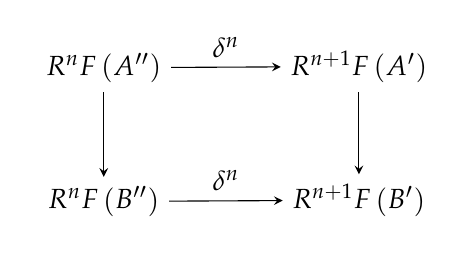
\begin{tikzpicture}
			\matrix (m) [matrix of math nodes,row sep=3em,column sep=4em,minimum width=2em]
			{
				R^nF\left(A''\right) & R^{n+1}F\left(A'\right)\\ 
				R^nF\left(B''\right) & R^{n+1}F\left(B'\right)\\};
			\path[-stealth]
			(m-1-1) edge node [above] {$\delta^n$} (m-1-2)
			(m-2-1) edge node [above]  {$\delta^n$} (m-2-2)
			(m-1-1) edge node [right]  {} (m-2-1)
			(m-1-2) edge node [right] {} (m-2-2);
		\end{tikzpicture}
		\\
		\	
		\item[(e)] For each injective object $I$ of $\mathfrak A$, and for each $n \ge 0$, we have $R^nF\left(I\right)= 0$.
		
	\end{enumerate}
\end{theorem}




\subsection{Algebras of foliations}

\subsubsection{Groupoid Preliminaries}
I will assume that the reader is familiar with the basic definitions of Lie groupoids. For this background, see \cite{mac3,cds-w,m-m,lan2}. I use the term ``Lie groupoid'', but the terms ``smooth groupoid'' and ``differential groupoid'' are also used synonymously in the literature. All groupoids here are Lie groupoids.

A Lie groupoid \emph{homomorphism} is a smooth map between Lie groupoids that is a functor if the groupoids are viewed as categories.

Given a groupoid $\G$, I denote by $\G_k\subset\G^k$ the $k$-nerve; that is, the set of composable chains of $k$ elements. The $0$-nerve $\G_0$ is the base manifold of $\G$, which I usually call $M$. I use the following notations for the structure maps of a generic groupoid. The unit is $\unit: M\into \G$, but I usually treat $M$ as a submanifold, unless I need to refer to the inclusion explicitly. The source and target maps are $\s,\t:\G\onto M$. The multiplication map is $\m:\G_2\onto\G$, but for a composable pair $(\gamma,\eta)\in\G_2$ I denote multiplication by apposition or a dot as $\gamma\eta=\gamma\cdot\eta=\m(\gamma,\eta)$. The inverse map is $\inv:\G\to\G$, but for $\gamma\in\G$ I denote its inverse as $\gamma^{-1}=\inv(\gamma)$. I also denote the Cartesian projections to the first and second factors of $\G^2$ as $\pr_1,\pr_2:\G_2\subset \G^2\onto\G$.

The nerve of a groupoid has a natural structure as a simplicial manifold. The maps $\s$, $\t$, $\m$, $\pr_1$, and $\pr_2$ are face maps.  This structure gives a simplicial coboundary operator $\partial^*$ on differential forms on the nerve, $\Omega^\bullet(\G_\bullet)$. In particular, for $\theta\in\Omega^\bullet(M)$,
\[
\partial^*\theta := \t^*\theta - \s^*\theta \in \Omega^\bullet(\G)
\]
and for $\omega\in\Omega^\bullet(\G)$,
\begin{subequations}
	\bean
	\partial^*\omega := \pr_1^*\omega - \m^*\omega + \pr_2^*\omega \in\Omega^\bullet(\G_2) .
	\eean
	
	\begin{definition}
		A differential form $\omega\in\Omega^\bullet(\G)$ is \emph{multiplicative} if
		\bean
		\partial^*\omega = 0 .
		\eean
		A \emph{symplectic groupoid} is a groupoid $\Sigma$ with a multiplicative symplectic form $\omega\in\Omega^2(\Sigma)$. (I usually denote a symplectic groupoid as $\Sigma$.)
	\end{definition}
	\label{multiplicative.form}
\end{subequations}

It will also be useful to extend the simplicial coboundary to line bundles, in a multiplicative sense. If $\Lambda$ is a line bundle over $M$ and $\G$ is a groupoid over $M$, then
\[
\partial^* \Lambda := \t^*\Lambda \otimes \s^*\Lambda^*
\]
is a line bundle over $\G$. If $L$ is a line bundle over $\G$, then 
\bean
\label{L_coboundary}
\partial^* L := \pr_1^* L \otimes \m^* L^* \otimes \pr_2^* L
\eean
is a line bundle over $\G_2$. This continues so that the coboundary of a line bundle over $\G_k$ is a line bundle over $\G_{k+1}$. The coboundary of a coboundary, $\partial^*\partial^* L$, is a canonically trivial line bundle. If $L$ is equipped with a connection, then $\partial^*L$ inherits a connection, and 
\[
\curv \partial^*L = \partial^*(\curv L) .
\]
A section of a line bundle $\sigma \in \Gamma(\G_k,L)$ has a multiplicative coboundary $\partial^*\sigma \in \Gamma(\G_{k+1},\partial^* L)$. 

It is standard terminology to use $\s$ as a prefix to describe a property of the fibers of $\s:\G\to M$. Hence $\G$ is \emph{$\s$-connected} if the fibers are connected, \emph{$\s$-simply connected} if they are simply connected, and \emph{$\s$-locally trivial} if they form a bundle. These properties are exactly the same as ``$\t$-connected'' \emph{et cetera}, but it is just conventional to refer to $\s$.

I also use a superscript to denote certain subbundles of the tangent bundle, namely $T^\s\G := \ker T\s \subset T\G$ and likewise $T^\t\G$ and $T^\m\G_2$.

I denote an arbitrary Lie algebroid over $M$ as $A$. Every Lie algebroid anchor map is denoted as $\#:A\to TM$. This includes the anchor map given by a Poisson structure $\#:T^*M\to TM$ and even the map given by the symplectic structure on a symplectic groupoid, $\# : T^*\Sigma \to T\Sigma$. When there is a real danger of confusion, I will use a subscript to indicate which anchor map it is.



%If $\Sigma$ is a symplectic groupoid with base manifold $M$, then $\omega$ induces a Poisson structure on $M$. For $f,g\in\C^\infty(M)$, the Poisson brackets are related by 
%\[
%\t^*\{f,g\} = \{\t^*f,\t^*g\}
%\]
%where $\t:\G\to M$ is the target map. Conversely, if $\G$ source connected, it is said to integrate the Poisson manifold $M$. 

%\subsection{Standard Constructions}
I denote by $\Alg$ the Lie functor from the category of Lie groupoids (and smooth homomorphisms) to the category of Lie algebroids, see \cite{mac3}. This restricts to the classical Lie functor from Lie groups to Lie algebras.

I denote by $\Grp$ the inverse of $\Alg$ (see \cite{c-f1}). The domain is the full subcategory of integrable Lie algebroids (i.e., the image of $\Alg$). If $A$ is an integrable Lie algebroid, then $\Grp(A)$ is the unique (up to isomorphism) $\s$-connected and $\s$-simply connected groupoid such that $A\cong \Alg\Grp(A)$. I call $\Grp(A)$ \emph{the} integration of $A$, but I will say that any $\s$-connected groupoid $\G$ with $\Alg(\G)\cong A$ \emph{integrates} $A$.

If $M$ is a Poisson manifold, then the cotangent bundle $T^*M$ with the Koszul bracket is a Lie algebroid. I will say that a symplectic groupoid over $M$ integrates $M$ if $\t$ is a Poisson map; $\Sigma$ is a symplectic integration of $M$ if and only if it is a groupoid integration of $T^*M$.
Any Lie groupoid integrating this has a natural symplectic groupoid structure. I will denote \emph{the} symplectic integration by $\Sig(M):=\Grp(T^*M)$ (see \cite{c-f2}).

Any manifold can be regarded as a groupoid, with every point a unit. Given a manifold, we can also construct the pair groupoid $\Pair(M):=M\times M$; note that this integrates $TM$. If $M$ happens to be a symplectic manifold, then the pair groupoid is a symplectic groupoid if we give it the symplectic structure of $M\times M^-$, where $M^-$ is $M$ with the symplectic form reversed. In this case $\Pair(M)$ is a symplectic integration of $M$.

For an arbitrary manifold, there is also the fundamental groupoid $\PI(M)$. This is the $\s$-simply connected cover of $\Pair(M)$, hence $\PI(M)=\Grp(TM)$. If $M$ is symplectic, then $\PI(M)$ inherits a symplectic groupoid structure from $\Pair(M)$, and $\Sig(M)=\PI(M)$.

Given a Lie groupoid $\G$ over $M$, we can construct another Lie groupoid simply by applying the tangent functor. The unit manifold of $T\G$ is $TM$, the source map is $T\s:T\G\to TM$, the multiplication is $T\m: T\G_2\to T\G$, \emph{et cetera}.  The complexified tangent bundle $T_\co\G$ is a groupoid in the same way. This tangent groupoid is very important for my definition of polarization, but it should not be confused with Connes' tangent groupoid \cite{con1}, which is also used in an example of quantization.

The cotangent bundle $T^*\G$ is a groupoid as well, but in a very different way. This is a symplectic groupoid over $\Alg^*(\G)$, the dual vector bundle of the Lie algebroid. This is an important example in Section~\ref{Linear}.

\subsubsection{Convolution}
There are two standard ways of constructing the convolution algebra of a Lie groupoid: using either a Haar system \cite{ren} or half-densities \cite{con1}. I favour the latter approach, because it is closer to the Hilbert space construction in geometric quantization. However, there is still an important discrepancy between half-forms and half-densities.

With this in mind, let's try to modify the definition of the convolution algebra by substituting half-forms for half-densities. This means using a bundle,
\bean
\label{half_form1}
\Omega^{1/2} := \sqrt{\Wedgem (T^{\t*}_\co\G\oplus T^{\s*}_\co\G)} .
\eean
If the bundle $T^\t\G\oplus T^\s\G$ is orientable, then there exists a preferred ``positive'' choice of square root, and with this choice, half-forms are equivalent to half-densities. This orientability condition is frequently satisfied; it is true if the Lie algebroid $\Alg(\G)$ is an orientable bundle or if $\G$ is $\s$-simply connected.

If some other choice of square root is chosen, then it may still define a convolution algebra. However, it will not generally be possible to complete this to a \cs-algebra. The potential problem is exemplified by the $*$-algebra of matrices on an indefinite inner product space; that is not a \cs-algebra.

The convolution product of $a,b\in\Gamma_{\mathrm c}(\G,\Omega^{1/2})$ is defined by integrating $\pr_1^*a \pr_2^*b$ over the fibers of $\m$. For $\gamma\in\G$, the fiber $\m^{-1}(\gamma)$ is explicitly parametrized as
\bean
\label{m_fiber}
\m^{-1}(\gamma) = \{(\eta,\eta^{-1}\gamma) \mid \eta \in \t^{-1}(\t \gamma)\} .
\eean
This gives the standard expression for the convolution product (see \cite{con1})
\bean
\label{convolution}
(a*b)(\gamma) := \int_{\eta\in\t^{-1}(\t\gamma)}  a(\eta) b(\eta^{-1}\gamma) .
\eean
To make sense of this expression, note that \eqref{m_fiber} implies isomorphisms
\[
T^\m\G_2 \cong \pr_1^* T^\t\G \cong \pr_2^* T^\s\G .
\]
Using these, the coboundary bundle (see \eqref{L_coboundary}) is
\[
\partial^*\Omega^{1/2} \cong \Wedgem T^{\m*}_\co\G_2 \cong \pr_1^*\Wedgem T^{\t*}_\co\G
\]
the bundle of volume forms along the fibers of $\m$ in $\G_2$. With this isomorphism, the product $\pr_1^* a \pr_2^* b$ is a section of 
\[
\m^* \Omega^{1/2} \otimes  \pr_1^*\Wedgem T^{\t*}_\co\G .
\]
So, integrating this over $\t^{-1}(\t\gamma)$ in \eqref{convolution} does give another section of $\Omega^{1/2}$.

The other important property of $\Omega^{1/2}$ is the canonical isomorphism
\[
\inv^*\Omega^{1/2} \cong \overline{\Omega^{1/2}} .
\]
This defines the involution on the convolution algebra.

\subsubsection{Twisted Convolution}
\label{Twisted}
The concept of twisted \cs-algebras of a groupoid is fairly standard. Let $L$ be a line bundle over $\G$ and $\sigma$ a cocycle with coefficients in $L$. In \cite{ren}, Renault mainly discusses the case where $L$ is trivial, but he gives a more general definition: $\cs(\G,\sigma)$ is the quotient of $\cs(\G^\sigma)$ induced by the fundamental representation of $\T$, where $\G^\sigma$ is the extended groupoid in \eqref{extension}. In order to generalize this to the polarized case, it is better to work with sections of  $L\otimes \Omega^{1/2}$, and this is easy enough.

For $a,b\in \Gamma_{\mathrm c}(\G,L\otimes \Omega^{1/2})$, the twisted convolution product is defined by modifying \eqref{convolution} to
\[
(a*b)(\gamma) := \int_{\eta\in\t^{-1}(\t\gamma)} \sigma(\eta,\eta^{-1}\gamma)\, a(\eta)\, b(\eta^{-1}\gamma) .
\]

Although this is constructed with a cocycle $\sigma$, the algebra only depends upon the cohomology class of $[\sigma]\in \Tw(\G)$. 


\begin{definition}
	% PAGE 11 (15)
	Suppose that $\mathscr C$ is some category. A map $p$ from a set $A$ onto a set $A^0$ such that
	each fiber $p^{-1} ( u )$ is an object of  $\mathscr C$ will be called a  $\mathscr C$-\textit{bundle} map and $A$ will be called  $\mathscr C$-bundle.  Let $A$ be
	a  $\mathscr C$ - bundle with the bundle map $p: A \to A_0$. Write $A_u \bydef p^{-1} ( u )$.
	$$
	\text{Iso}(A) = \left\{\text{isomorphisms }\phi_{u,v}| A_u\to A_v\quad u,v \in A^0\right\} 
	$$	
	has a natural structure of groupoid. %: #u,v and ~ v ' , ware composable i f f v' = v - then t h e i r product is ~u,v  #v,w' and 4 -1 is the iso-' U~Vmorphism inverse of ~u,v" The b i j e c t i o n idu, u ~ u i d e n t i f i e s the u n i t space of Iso(A)and A O. Iso(A) is c a l l e d the isomorphism groupoid of the C-bundle A.
\end{definition}
\begin{definition}
	% Definition 1.11.
	Let $\G$ be a groupoid. A $\G$-\textit{bundle} $(A,L)$ is a $\mathscr C$ - bundle $A$ together
	with a homomorphism $L : G \to \text{Iso} (A)$ such that $L^0: \G^0\to A^0$ is a bijection . (We will often identify $\G^0$ and $A^0$). When  $\mathscr C$  is the category of Abelian groups, one speaks of a
	$\G$-\textit{module bundle}.
\end{definition}
\begin{empt}\label{groupoig_gn_empt}
	Given a $\G$-module bundle $( A , L )$, one can form the following cochain complex. Let
	us first define $\G^n$ for any $n\in\N$. The sets $\H^0$ , $\G^1\bydef \G$ and $\G^2$ have already been defined. For $n> 2$, $\quad \G^n$ is the set of $n$-tuples $(x_0 . . . . . x_{n-1}) \in \G\times...\times \G$ such that for $
	j = 1 , . . . , n - 1$ , $\quad x_j$ is composable with its left  neighbor. A $n$-cochain is a function from $G^n$ to $A$ which satisfies the conditions
	\begin{enumerate}
		\item[(i)] $p\circ f(x_0 . . . . . x_{n-1}) = d(x_0)$ and
		\item[(ii)] if $n > 0$ and for some $j = 0, . . . , n - 1$ , $\quad x_0 \in \G^0$, then $f ( x_0, ..., x_j , ..., x_{n-1})\in A^0$.
	\end{enumerate}
	The set $C^n\left(\G, A\right)$ of $n$-cochains is an Abelian group under point-wise addition. The
	sequence 
	\bean
	0 \to C^0\left( \G, A\right)\to C^0\left( \G, A\right)\to C^1\left( \G, A\right)\to...\to  C^n\left( \G, A\right) \xrightarrow{\delta^n} C^{n + 1}\left( \G, A\right)\to ...
	\eean
	where 
	\be\label{groupoid_b_eqn}
	\begin{split}
		\delta^0f(x)\bydef L(x)\quad  f\circ s(x) - f \circ r ( x ),\\
		\delta^n(f(x_0 ,..., x_n) = L ( x_0 ) f ( x_1,..., x_n) +\\+ \sum_{j=1}^n (-1)^j
		f ( x_0 ,..., x_{j-1}x_j . . . . . x_{n-1})+(-1)^{n-1} f ( x_0 , . . . , x_{n-1}) \quad  n > 0,
	\end{split}
	\ee
	
	is a cochain complex.
\end{empt}	
\begin{definition}\label{groupoid_cocycle_defn}
	The group of $n$-cocycles of this complex will be denoted by $Z^n(\G,A)$,
	the group of $n$-coboundaries will be denoted by $B^n(\G,A)$ and the $n$-th cohomology group
	$Z^n(\G,A)/B^n(\G,A)$ will be denoted by $H^n(\G,A)$.
\end{definition}
\paragraph{}
Let $\G$ be a locally compact Hausdorff groupoid with left  Haar system $\left\{\la^u\right\}$ and let $\sigma$ be a continuous 2-cocycle in $Z^2\left(\G, \T\right)$. For $f ,g \in C_c(\G, \sigma )$, let us define
\be\label{groupoid_*_c_eqn}
\begin{split}
	f * g \left(x\right)\bydef 
	\int f ( x y ) g \left( y^{-1}\right)\sigma\left(xy, y^{-1} \right) d\la^{d(x)}(y),\\
	f^* ( x ) \bydef \overline{f ( x^{ -1})}~\overline{\sigma\left(x, x^{-1} \right)}, 	
\end{split}
\ee	
In particular is $\sigma$ is trivial then one has a $*$-algebra
\be\label{groupoid_*_eqn}
\begin{split}
	f * g \left(x\right)\bydef 
	\int f ( x y ) g \left( y^{-1}\right) d\la^{d(x)}(y),\\
	f^* ( x ) \bydef\overline{f ( x^{ -1})} 	
\end{split}
\ee	
which is a specialization of \eqref{groupoid_*_c_eqn}

\begin{empt} % ??? DEFINE NORM ???
	Let $\G$ be a locally compact groupoid with left  Haar system $\left\{\la^u\right\}$ (cf. Definition \ref{groupoid_haar_defn}).  For $f$ and $g\in C_c\left(\G\right)$, let  us define
	\be\label{groupoid_*__defn}
	\begin{split}
		f * g \left(x\right)\bydef 
		\int  f ( x y ) g \left( y^{-1}\right) d\la^{d(x)}(y),\\
		f^* ( x ) \bydef\overline{f ( x^{ -1})} 	
	\end{split}
	\ee
	It is proven in \cite{renault:gropoid_ca} that the equations yield a $*$-algebra. 
\end{empt}
\begin{definition}\label{groupoid_representation_defn}\cite{renault:gropoid_ca}
	%1.3. D e f i n i t i o n : 
	A \textit{representation} of $C_c\left(\G, \sigma\right)$ on a Hilbert space $\H$ is a $*$-homomorphism $L : C_c\left(\G, \sigma\right) \to B\left(\H \right)$ which is continuous when $C_c\left(\G, \sigma\right)$ has the inductive limit 
	topology (cf. Definition \ref{top_ind_lim_defn}) and $B\left(\H \right)$  the weak operator topology (cf. Definition \ref{weak_topology_defn}), and is such that the linear  span of
	$$
	L\left(f \right) \xi , \quad f \in C_c\left(\G, \sigma\right), \quad \xi \in \H
	$$
	is dense in $\H$.
\end{definition}
\begin{lemma}\label{groupoid_mult_repr_lem}\cite{renault:gropoid_ca}
	%1.13. Lemma : 
	If $L$ is a representation of $C_c\left(\G, \sigma\right)$, there exists a unique representation
	$M$ of $C_c\left(\G^0\right)$ such that for every $h \in C_c\left(\G^0\right)$ and every $f\in C_c\left(\G, \sigma\right)$, $L\left(h f \right)= M\left(h \right)L\left(f \right)$  and
	$L\left(fh \right)= L\left(f \right)M\left(h \right)$. 
\end{lemma}
\begin{definition}\label{groupoid_red_defn}	\cite{renault:gropoid_ca}%2.8. Definition : 
	The \textit{reduced $C^*$ -algebra} $C^*_r\left(\G, \sigma \right)$ of $\G$ is the completion of
	$C^*_r\left(\G, \sigma \right)$ for the reduced norm $\left\|\cdot  \right\|_r$.
\end{definition}

\section*{Acknowledgment}


\paragraph*{}
 Author would like to acknowledge members of the Moscow State University Seminars
"Noncommutative geometry and topology", "Algebras in analysis" leaded by professors A. S. Mishchenko and  A. Ya. Helemskii for a discussion
of this work. 


\begin{thebibliography}{10}
		\bibitem{arveson:c_alg_invt} W. Arveson. {\it An Invitation to $C^*$-Algebras}, Springer-Verlag. ISBN 0-387-90176-0, 1981.
		
\bibitem{blackadar:ko} B. Blackadar. {\it K-theory for Operator Algebras}, Second edition. Cambridge University Press. 1998.
	
		\bibitem{bredon:sheaf} Bredon, Glen E. (1997), \textit{Sheaf theory}. Graduate Texts in Mathematics, 170 (2nd ed.), Berlin, New York: Springer-Verlag.  ISBN 978-0-387-94905-5, MR 1481706 (oriented towards conventional topological applications), 1997.
		
\bibitem{bourbaki_sp:gt} N. Bourbaki, {\it Elements of Mathematics. General Topology}, Part 1. \newline HERMANN, \'{E}DITEURS DES SCIENCES ET DAS ARTS \newline 115 Boulevard Saint-Germain. Paris \newline ADDISON-WESLEY PUBLISHING COMPANY. \newline Reading, Massachusets - Palo Ito - London - Don Mills, Ontario \newline A translation of \newline \'{E}L\'{E}MENTS DE MATH\'{E}MATIQUE, TOPOLOGIE G\'{E}N\'{E}RALE, \newline originally published in French by Hermann, Paris. 1966.

\bibitem{candel:foliI}Alberto Candel, Lawrence Conlon. \textit{Foliations I}. Graduate Studies in Mathematics, American Mathematical Society (1999), 1999.


\bibitem{candel:foliII}Alberto Candel, Lawrence Conlon. \textit{Foliations II}. American Mathematical Society; 1 edition (April 1 2003), 2003.

\bibitem{godement:sheaf} Roger Godement, \textit{Topologie Alg�brique et Th�orie des Faisceaux}. Actualit�s Sci. Ind. No. 1252. Publ. Math. Univ. Strasbourg. No. 13 Hermann, Paris. 1958.


	
%\bibitem{connes:ncg94} Alain Connes. {\it Noncommutative Geometry}, Academic Press, San Diego, CA,  661 p., ISBN 0-12-185860-X, 1994.

	\bibitem{hartshorne:ag} Robin Hartshorne. {\it Algebraic Geometry.} Graduate Texts in Mathematics, Volume 52, 1977.
	
	\bibitem{hatcher:at}Allen Hatcher, \textit{Algebraic topology}. Cambridge University Presses, Cambridge, 2002. 
	 	
	\bibitem{johnstone:stone_spaces} Peter Johnstone. \textit{Stone Spaces} Cambridge Studies in Advanced Mathematics 3, Cambridge University Press (1982, 1986).
	
	\bibitem{johnstone:topos}Peter Johnstone. \textit{Topos Theory}, L. M. S. Monographs no. 10, Academic Press 1977.
	
			\bibitem{matro:hcm} Manuilov V.M., Troitsky E.V. \textit{Hilbert $C^*$-modules}. % Publication Year: 2005. ISBN-10: 0-8218-3810-5 ISBN-13: 978-0-8218-3810-5 
	Translations of Mathematical Monographs, vol. 226, 2005.

\bibitem{miyazaki_cw} Hiroshi Miyazaki, {The paracompactness of CW-complexes}, Tohoku Math. J. (2) Volume 4, Number 3 (1952), 309-313. 1952 	
	
\bibitem{munkres:topology} James R. Munkres. {\it Topology.} Prentice Hall, Incorporated, 2000.
	
	\bibitem{murphy}G.J. Murphy. {\it $C^*$-Algebras and Operator Theory.} Academic Press 1990.	
		\bibitem{pedersen:ca_aut}Gert K Pedersen. {\it $C^*$-algebras and their automorphism groups}. London ; New York : Academic Press, 1979.

%\bibitem{pedersen:mea_c} Gert K Pedersen.  \textit{Measure Theory for $C^*$-Algebras}. Mathematica Scandinavica (1966) Volume: 19, page 131-145 ISSN: 0025-5521; 1903-1807/e, 1966.
	
	
	\bibitem{rae:ctr_morita} Iain Raeburn, Dana P. Williams. \textit{Morita Equivalence and Continuous-trace $C^*$-algebras}. American Mathematical Soc., 1998.


\bibitem{renault:gropoid_ca} Jean Renault, \emph{A groupoid approach to {$C\sp{\ast} $}-algebras}, Lecture Notes in Mathematics, vol. 793, Springer, Berlin, 1980. 
%\bibitem{rudin:fa}Walter Rudin. \textit{Functional Analysis}, Second Edition, McGraw-Hill, Inc. New York St. Louis San Francisco Auckland Bogota Caracas Hamburg Lisbon London Madrid Mexico Milan Montreal New Delhi Paris San Juan Sao Paulo Singapore Sydney Tokyo Toronto, 1991.



	
		\bibitem{spanier:at}
E.H. Spanier. {\it Algebraic Topology.} McGraw-Hill. New York. 1966.

		\bibitem{thomsem:ho_type_uhf} Klaus Thomsen. {\it The homotopy type of the group of automorphisms of a $UHF$-algebra}. Journal of Functional Analysis. Volume 72, Issue 1, May 1987.

\end{thebibliography}



	\end{document}
